%% =====================================================================
%%  M.Tech Project Report  -  Vadithe Sai Kumar Naik (CS25M053)
%%  PDDL-Based Mission Planning for a Drone Swarm Simulator
%%  Department of Computer Science and Engineering, IIT Madras
%%
%%  Build:  pdflatex main.tex   (run twice so contents and lists update)
%%          or  tectonic main.tex
%%  Files: figures/iitm_logo.png and figures/*_sample.pdf
%% =====================================================================
\documentclass[11pt,a4paper,oneside]{report}

%% ---------- Personal details (edit here) ----------------------------
\newcommand{\thesistitle}{PDDL-Based Mission Planning for a Drone Swarm Simulator}
\newcommand{\thesistitlebreak}{PDDL-Based Mission Planning for a\\ Drone Swarm Simulator}
\newcommand{\authorname}{Vadithe Sai Kumar Naik}
\newcommand{\rollno}{CS25M053}
\newcommand{\submitdate}{December 2026}
\newcommand{\advisor}{Dr. N. S. Narayanaswamy}
\newcommand{\coadvisor}{Dr. Jaimandeep Singh}

%% ---------- Packages -------------------------------------------------
\usepackage{iftex}
\ifXeTeX
  \usepackage{newtxtext,newtxmath}
  \setmonofont[Scale=0.95,BoldFont=Inconsolatazi4-Bold.otf]{Inconsolatazi4-Regular.otf}
\else
  \usepackage[T1]{fontenc}
  \usepackage[utf8]{inputenc}
  \usepackage{newtxtext,newtxmath}
  \usepackage[varqu,scaled=0.95]{zi4}
\fi
\usepackage{xstring}
\usepackage[a4paper,top=1in,bottom=1in,left=1.2in,right=1in]{geometry}
\usepackage{setspace}
\setstretch{1.22}
\setlength{\emergencystretch}{3em}
\clubpenalty=10000 \widowpenalty=10000 \displaywidowpenalty=10000
\raggedbottom
\renewcommand{\arraystretch}{1.18}
\usepackage{graphicx}
\usepackage{booktabs,tabularx,array,multirow,longtable}
\newcolumntype{Y}{>{\raggedright\arraybackslash}X}
\newcolumntype{P}[1]{>{\raggedright\arraybackslash}p{#1}}
\usepackage{enumitem}
\setlist{itemsep=1pt,topsep=4pt}
\usepackage[table]{xcolor}
\usepackage{amsmath}
\usepackage{listings}
\usepackage{tikz}
\usetikzlibrary{arrows.meta,positioning,shapes.geometric,shapes.misc,fit,calc,backgrounds,decorations.pathreplacing}
\usepackage{pgfplots}
\pgfplotsset{compat=1.17}
\usepackage[font=small,labelfont=bf,labelsep=colon]{caption}
\captionsetup[table]{justification=raggedright,singlelinecheck=false,skip=6pt}
\captionsetup[figure]{format=hang,skip=6pt}
\usepackage{titlesec}
\usepackage{titletoc}
\usepackage{float}
\usepackage{needspace}
\usepackage{adjustbox}
\usepackage{microtype}
\usepackage[section]{placeins}
\usepackage{xurl}
\usepackage[hidelinks]{hyperref}
\hypersetup{
  pdftitle={\thesistitle},
  pdfauthor={\authorname},
  pdfsubject={M.Tech thesis, IIT Madras}
}

%% ---------- Colours --------------------------------------------------
\definecolor{navy}{HTML}{0F2240}
\definecolor{amber}{HTML}{F0A30A}
\definecolor{codebg}{HTML}{F5F5F5}
\definecolor{coderule}{HTML}{C8C8C8}
\definecolor{kwblue}{HTML}{1F5FBF}
\definecolor{cmtgray}{HTML}{7A7A7A}
\definecolor{okgreen}{HTML}{2E7D32}
\definecolor{warnred}{HTML}{C62828}
\definecolor{softblue}{HTML}{E8EEF7}
\definecolor{softamber}{HTML}{FDF1D8}

%% ---------- Chapter and section headings ----------------------------
\titleformat{\chapter}[display]
  {\centering\bfseries}
  {\LARGE\chaptertitlename\ \thechapter}
  {1.6em}
  {\huge}
\titlespacing*{\chapter}{0pt}{10pt}{28pt}
\titleformat{name=\chapter,numberless}[block]
  {\centering\bfseries\huge}{}{0pt}{}
\titlespacing*{name=\chapter,numberless}{0pt}{10pt}{24pt}
\titleformat{\section}{\bfseries\Large}{\thesection}{0.6em}{}
\titleformat{\subsection}{\bfseries\large}{\thesubsection}{0.6em}{}
\titleformat{\paragraph}[runin]{\bfseries}{}{0pt}{}[.]
\titlespacing*{\section}{0pt}{20pt}{10pt}
\titlespacing*{\subsection}{0pt}{14pt}{6pt}
\setcounter{secnumdepth}{3}
\setcounter{tocdepth}{2}

%% ---------- Contents, list of tables, list of figures ---------------
\renewcommand{\contentsname}{Contents}
\renewcommand{\listtablename}{List of Tables}
\renewcommand{\listfigurename}{List of Figures}
\titlecontents{chapter}[0pt]
  {\addvspace{0.65em}\bfseries\small}
  {\contentslabel{2.3em}}{}{\titlerule*[0.7pc]{.}\contentspage}
\titlecontents{section}[2.8em]
  {\small\addvspace{0.12em}}{\contentslabel{2.8em}}{}
  {\titlerule*[0.7pc]{.}\contentspage}
\titlecontents{subsection}[6em]
  {\small}{\contentslabel{3.2em}}{}{\titlerule*[0.7pc]{.}\contentspage}
\titlecontents{figure}[3em]
  {\small\addvspace{0.25em}}{\contentslabel{3em}}{}
  {\titlerule*[0.7pc]{.}\contentspage}
\titlecontents{table}[3em]
  {\small\addvspace{0.25em}}{\contentslabel{3em}}{}
  {\titlerule*[0.7pc]{.}\contentspage}
% Front-matter entries in the contents (bold, upper case, no dots)
\newcommand{\addfront}[1]{%
  \addtocontents{toc}{\protect\noindent\protect\rule{0pt}{1.5em}\protect\textbf{#1}\protect\hfill\protect\textbf{\thepage}\protect\par}}

%% ---------- Code listings (PDDL) -------------------------------------
\lstdefinelanguage{PDDL}{
  morekeywords=[1]{define,domain,problem,and,or,not,forall,exists,when,imply,
    increase,decrease,assign,either},
  morekeywords=[2]{:requirements,:types,:predicates,:functions,:action,
    :parameters,:precondition,:effect,:objects,:init,:goal,:domain,:strips,
    :typing,:numeric-fluents,:negative-preconditions,:conditional-effects,
    :equality,:disjunctive-preconditions,:universal-preconditions},
  sensitive=false,
  morecomment=[l]{;},
  alsoletter={:-},
}
\lstset{
  language=PDDL,
  basicstyle=\ttfamily\footnotesize\setstretch{1.0},
  keywordstyle=[1]\color{kwblue}\bfseries,
  keywordstyle=[2]\color{kwblue},
  commentstyle=\color{cmtgray}\itshape,
  backgroundcolor=\color{codebg},
  frame=single,
  rulecolor=\color{coderule},
  framesep=4pt,
  xleftmargin=6pt,xrightmargin=6pt,
  aboveskip=8pt,belowskip=8pt,
  breaklines=true,
  breakatwhitespace=true,
  columns=fullflexible,
  keepspaces=true,
  showstringspaces=false,
  tabsize=4,
}
\lstdefinestyle{plain}{language={},keywordstyle=,commentstyle=}
\lstdefinestyle{appendix}{basicstyle=\ttfamily\scriptsize\setstretch{1.0},
  numbers=left,numberstyle=\tiny\color{cmtgray},numbersep=6pt,xleftmargin=18pt}

\newcommand{\code}[1]{\texttt{#1}}
\newcommand{\cmd}[1]{\mbox{\texttt{#1}}}
\newcommand{\recordlabel}[1]{\par\smallskip\noindent\hspace*{1.2em}\textit{#1}\par}

%% ---------- Reusable TikZ styles -------------------------------------
\tikzset{
  drone/.style={circle,fill=navy,minimum size=7pt,inner sep=0pt},
  leader/.style={circle,fill=amber,minimum size=9pt,inner sep=0pt},
  link/.style={navy,line width=0.7pt},
  box/.style={draw=navy,line width=0.8pt,rounded corners=3pt,fill=softblue,
              align=center,font=\small,inner sep=5pt,minimum height=2.2em},
  abox/.style={box,fill=softamber,draw=amber!80!black},
  gbox/.style={box,fill=white},
  arr/.style={-{Stealth[length=5pt]},line width=0.8pt,navy},
  darr/.style={arr,dashed},
}

\begin{document}
\hypersetup{pageanchor=false}

%% =====================================================================
%%  COVER PAGE
%% =====================================================================
\begin{titlepage}
\setstretch{1.05}
\thispagestyle{empty}
\noindent\begin{minipage}[c]{0.36\textwidth}
  
\includegraphics[width=0.62\linewidth]{figures/iitm_logo.png}
\end{minipage}%
\begin{minipage}[c]{0.64\textwidth}
  \setstretch{1.05}\small
  DEPARTMENT OF COMPUTER SCIENCE AND\\
  ENGINEERING\\
  INDIAN INSTITUTE OF TECHNOLOGY MADRAS\\
  CHENNAI -- 600036
\end{minipage}

\vspace{0.6cm}
\noindent\rule{\textwidth}{2pt}

\vspace{1.0cm}
\begin{center}
  {\setstretch{1.2}\LARGE\bfseries \thesistitlebreak\par}

  \vspace{0.8cm}
  % PDDL-based planning illustration (editable vector artwork).
  \begin{adjustbox}{max width=\linewidth,max height=5.8cm}
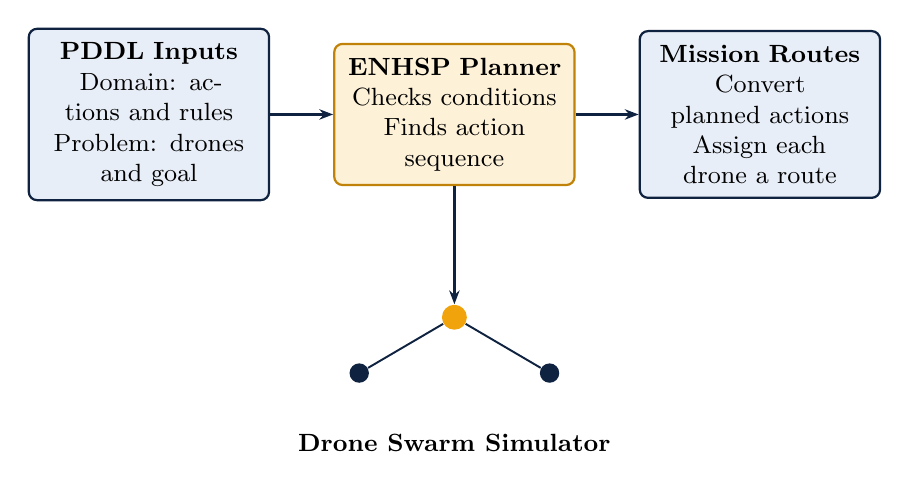
\begin{tikzpicture}[node distance=9mm and 8mm]
\node[box,text width=2.7cm] (d) {\textbf{PDDL Inputs}\\Domain: actions and rules\\Problem: drones and goal};
\node[abox,right=of d,text width=2.7cm] (e) {\textbf{ENHSP Planner}\\Checks conditions\\Finds action sequence};
\node[box,right=of e,text width=2.7cm] (r) {\textbf{Mission Routes}\\Convert planned actions\\Assign each drone a route};
\draw[arr] (d)--(e);\draw[arr] (e)--(r);
\node[leader,below=15mm of e] (l) {};
\node[drone,below left=5mm and 10mm of l] (a) {};
\node[drone,below right=5mm and 10mm of l] (b) {};
\draw[arr] (e)--(l);\draw[link] (a)--(l)--(b);
\node[font=\small,below=12mm of l] {\textbf{Drone Swarm Simulator}};
\end{tikzpicture}
\end{adjustbox}

  \vspace{0.9cm}
  {\itshape A Thesis\par}
  \vspace{0.25cm}
  {\itshape Submitted by\par}
  \vspace{0.3cm}
  {\Large\bfseries \authorname\par}
  \vspace{0.5cm}
  {\itshape For the award of the degree\par}
  \vspace{0.25cm}
  {\itshape Of\par}
  \vspace{0.25cm}
  {\bfseries MASTER OF TECHNOLOGY\par}
  \vspace{0.2cm}
  \submitdate
\end{center}
\end{titlepage}

%% =====================================================================
%%  THESIS CERTIFICATE
%% =====================================================================
\thispagestyle{empty}
\begin{center}
  {\LARGE\bfseries Thesis Certificate\par}
\end{center}
\vspace{0.8cm}
\noindent This is to certify that the thesis entitled \textbf{\thesistitle}, submitted by
\textbf{\authorname\ (\rollno)} to the Indian Institute of Technology Madras in partial
fulfilment of the requirements for the degree of \textbf{Master of Technology}, is a bona fide
record of the work carried out under the guidance of \textbf{\advisor}, Project Advisor, and
\textbf{\coadvisor}, Project Co-Advisor.

\noindent The contents of this thesis, in full or in part, have not been submitted to any other
institute or university for the award of a degree or diploma.

\vspace{2.2cm}
\noindent
\begin{minipage}[t]{0.5\textwidth}
  \setstretch{1.15}
  Chennai 600036\\
  Date: \submitdate
\end{minipage}%
\begin{minipage}[t]{0.5\textwidth}
  \raggedleft\setstretch{1.15}
  \textbf{\authorname}\\
  \rollno
\end{minipage}

\vspace{2.6cm}
\begin{flushright}
  \setstretch{1.15}
  \textbf{\advisor}\\
  Project Advisor, Professor\\
  Department of Computer Science and Engineering\\
  Indian Institute of Technology Madras
\end{flushright}

\vspace{1.8cm}
\begin{flushright}
  \setstretch{1.15}
  \textbf{\coadvisor}\\
  Project Co-Advisor\\
  Department of Computer Science and Engineering\\
  Indian Institute of Technology Madras
\end{flushright}

\vfill
\noindent{\small \textcopyright\ 2026 Indian Institute of Technology Madras}
\clearpage

%% =====================================================================
%%  FRONT MATTER
%% =====================================================================
\pagenumbering{roman}
\hypersetup{pageanchor=true}
\pagestyle{plain}

\addtocontents{toc}{\protect\noindent\protect\hfill\protect\textbf{Page}\protect\par}
\addtocontents{lot}{\protect\noindent\protect\makebox[4.2em][l]{\protect\textbf{Table}}\protect\hfill\protect\textbf{Caption}\protect\hfill\protect\textbf{Page}\protect\par\protect\vspace{0.6em}}
\addtocontents{lof}{\protect\noindent\protect\makebox[4.2em][l]{\protect\textbf{Figure}}\protect\hfill\protect\textbf{Caption}\protect\hfill\protect\textbf{Page}\protect\par\protect\vspace{0.6em}}
\chapter*{Acknowledgements}
\addfront{ACKNOWLEDGEMENTS}
I would like to express my sincere gratitude to my project advisor,
\textbf{\advisor}, and my project co-advisor, \textbf{\coadvisor}, for their
valuable guidance, patient support and encouragement throughout this project.
Their suggestions helped me develop clear PDDL models, understand the planning
results and improve the presentation of this work.

I thank the Department of Computer Science and Engineering at the Indian
Institute of Technology Madras for providing the facilities and academic
environment needed to carry out this project.

I am grateful to my project teammates for their cooperation and useful
discussions while integrating mission planning with the drone swarm simulator.
Working together also helped me contribute to parts of the graphical interface
and understand how a planned mission becomes a simulated flight.

Finally, I thank my family and friends for their constant encouragement and
support during the project and the preparation of this report.

\begin{flushright}
\textbf{\authorname}\\
\rollno\\
December 2026
\end{flushright}

\chapter*{Abstract}
\addfront{ABSTRACT}
\noindent\textbf{Keywords:} automated planning; PDDL; numeric planning; ENHSP; drone swarm;
formation flight; fault handling; battery management.

\medskip
A drone swarm mission is more than a route. Before a drone may take off, join a formation or
continue a leg, its battery must cover the next move, its GPS and radio links must work, its
health must be acceptable and its neighbours in the formation must be in place. This thesis
describes the planning layer of a software-in-the-loop drone swarm simulator, in which these
rules are written in the Planning Domain Definition Language (PDDL) and solved by the
Expressive Numeric Heuristic Search Planner (ENHSP). In this work, I developed the PDDL mission-planning models and contributed to
parts of the graphical interface used to prepare missions.

Ten mission plans were developed, each as a domain file and a problem template: point-to-point
travel, forest area search, V formation, two-dimensional grid formation, three-dimensional
(cube) grid formation, parabola formation, figure-eight train formation, star drone show,
planetary orbit show and road inspection. Every plan shares one vocabulary of drone states,
health flags, failure states and numeric fluents for battery, energy, altitude and health. A
plan service retargets each template onto the points the operator picks on the map, expands it
to the number of selected drones and passes it to ENHSP. Only the leader corridor is usually
planned symbolically; the other drones' routes are then derived geometrically from their
formation slots.

Inter-drone communication is modelled in two layers. In PDDL, each formation declares which
drones are neighbours and every formation action checks a per-drone \code{neighbor-comm-ok}
flag; the parabola plan goes further and requires each directed link to be established within
a communication range. At run time the ground station talks to each drone over a JSON-over-UDP
protocol with heartbeats, and formation keeping for trains and shows runs on board each drone
against a shared, time-stamped pace. Four fault types are modelled in the domains -- GPS loss,
communication loss, neighbour-link loss and health failure -- together with ground-controller
responses such as return, hover and sacrifice. Battery health is handled both as a planning
resource (energy per metre, climb and leg energy, a 30-unit reserve) and at run time through
low (20\,\%) and critical (5\,\%) thresholds that pause the swarm and ask the operator to decide.

The mission templates are adapted to the selected number of drones wherever
the mission supports expansion. Travel accepts one or more drones, search at
least two, V formation odd counts from three, grid formation at least four and
cube formation at least eight. Cube planning has been demonstrated up to
64 drones; this is an observed example, not a general upper bound. Figure-eight
capacity depends on the chosen path: the illustrated configuration supports
up to 27 drones. The star show supports 6--40 drones and the planetary show
supports 2--8. The current parabola mission uses exactly three active drones,
and road inspection uses one. These mission-specific limits make clear where
dynamic swarm sizing is supported and where the present implementation remains
fixed. Planning cost, communication assumptions and the absence of automatic
replanning after a failure remain limitations of this work.

\tableofcontents

\clearpage
\addfront{LIST OF TABLES}
\listoftables
\clearpage
\addfront{LIST OF FIGURES}
\begingroup\setstretch{1.0}\listoffigures\endgroup

\chapter*{Abbreviations}
\addfront{ABBREVIATIONS}
\begin{center}
\begin{tabular}{@{}p{0.22\textwidth}p{0.68\textwidth}@{}}
\toprule
\textbf{Abbreviation} & \textbf{Meaning} \\
\midrule
PDDL   & Planning Domain Definition Language \\
ENHSP  & Expressive Numeric Heuristic Search Planner \\
GCS    & Ground Control Station \\
GUI    & Graphical User Interface \\
UAV    & Unmanned Aerial Vehicle \\
SYSID  & MAVLink system identifier of a drone \\
MAVLink& Micro Air Vehicle Link, a lightweight drone messaging protocol \\
SITL   & Software in the Loop \\
UDP    & User Datagram Protocol \\
JSON   & JavaScript Object Notation \\
OSRM   & Open Source Routing Machine \\
AIBR   & Additive Interval Based Relaxation (ENHSP preprocessing) \\
RTL    & Return to Launch \\
\bottomrule
\end{tabular}
\end{center}

\clearpage
\pagenumbering{arabic}

%% =====================================================================
%%  CHAPTER 1  INTRODUCTION
%% =====================================================================
\chapter{Introduction}

\section{Background and Motivation}
Small unmanned aerial vehicles are now used for search, inspection, mapping and public light
shows. Many of these tasks are done better by a group of drones than by one drone. A group,
however, needs coordination. Each drone must know when to take off, which place in the
formation it must hold, which other drones it must stay in contact with, and what to do when
something goes wrong. Writing these rules directly in flight code makes them hard to read, hard
to check and hard to change.

Automated planning offers a cleaner way. In planning, the rules of the world are written once as
a \emph{domain}: a set of actions, each with the conditions under which it may be applied and the
changes it causes. A particular mission is written as a \emph{problem}: the drones, the places,
the starting state and the goal. A general-purpose planner then searches for a sequence of
actions that reaches the goal while respecting every rule. PDDL is the standard language for
writing such domains and problems.

This project is part of a larger drone swarm simulator built in the department. The simulator
runs each drone as an independent thread and offers a ground station GUI with a map, telemetry and fault injection. The work
reported here is the planning layer of that simulator: the PDDL models for every mission type,
and their link to the rest of the system.

\section{Problem Statement and Objectives}
The central problem is to express swarm missions -- including formations, communication
requirements, battery limits and failures -- in PDDL in a way that a numeric planner can solve
quickly for realistic swarm sizes, and whose plans can be turned into flyable routes. The work
had the following objectives:
\begin{enumerate}
  \item Design a common PDDL vocabulary for drone state, health, communication, battery and
        failure that every mission plan can share.
  \item Build domain and problem files for a range of missions: travel, area search, rigid
        formations (V, grid, cube, parabola), path-following trains (figure-eight), shape-changing
        shows (star, planets) and road inspection.
  \item Model drone-to-drone communication, so that a formation can only form and fly while the
        required links are up.
  \item Model faults (GPS, communication, neighbour link, health) and battery health, together
        with the ground controller's responses.
  \item Integrate the plans with the simulator, so that a plan is retargeted to the operator's map
        inputs, solved by ENHSP and executed by the drones, and verify the results.
\end{enumerate}

\section{Scope and Contributions}
In this work, I developed the PDDL mission-planning layer and contributed to parts of
the graphical interface. The main planning contributions are:
\begin{itemize}
  \item mission models for the supported tasks (Table~\ref{tab:inventory}),
        written using shared predicates and numeric fluents;
  \item a set of modelling patterns that keep formation problems tractable for large swarms:
        planning only the leader corridor, descriptive neighbour relations with per-drone
        communication flags, and propositional rather than numeric gates for ordered launches;
  \item a two-level model of communication: symbolic neighbour links in PDDL, including an
        explicit range-checked link model in the parabola plan, and the run-time protocol used
        by the ground station and the drones;
  \item a fault and battery model covering four failure types, ground-controller responses and
        energy accounting for travel, climb, cruise and hover;
  \item verification of every plan through the real planning pipeline, including scalability
        measurements and a record of the modelling defects found and fixed.
\end{itemize}

This report focuses on the PDDL models, their integration with mission preparation,
and their verification in the simulator. My contribution also includes parts of the GUI.
Physical flight tests are outside the scope of this work; the reported observations
come from simulation.

\section{Organisation of the Report}
Chapter~\ref{ch:background} reviews automated planning, PDDL, numeric planning and related work
on multi-drone missions. Chapter~\ref{ch:arch} explains the simulator architecture and the
planning pipeline. Chapter~\ref{ch:model} presents the common PDDL vocabulary and design
patterns. Chapter~\ref{ch:plans} describes all ten mission plans. Chapter~\ref{ch:comm}
explains how drones communicate, both in the model and at run time. Chapter~\ref{ch:faults}
covers fault modelling and battery health. Chapter~\ref{ch:results} reports the verification
results and the defects found. Chapter~\ref{ch:discussion} discusses limitations, and
Chapter~\ref{ch:conclusion} concludes with future work. Selected PDDL excerpts
are explained alongside the corresponding missions in Chapter~\ref{ch:plans}.

%% =====================================================================
%%  CHAPTER 2  BACKGROUND AND LITERATURE REVIEW
%% =====================================================================
\chapter{Background and Literature Review}\label{ch:background}

\section{Automated Planning}
Classical planning studies how an agent can reach a goal from a known initial state by applying
actions with known effects. A planning task is described by a set of
state variables, a set of actions and a goal. Each action has a \emph{precondition} that must
hold before it is applied and an \emph{effect} that changes the state. A \emph{plan} is a sequence
of actions that, applied in order from the initial state, ends in a state that satisfies the
goal. Heuristic search planners find such plans by estimating, for each state, how far it is
from the goal and expanding the most promising states first.

\section{The Planning Domain Definition Language}
PDDL was introduced to give planning competitions a common input
language. A PDDL model is split into two files:
\begin{itemize}
  \item the \textbf{domain} defines object types, \emph{predicates} (true/false facts such as
        \code{(gps-ok ?d)}), \emph{functions} (numeric values such as \code{(battery ?d)}) and
        \emph{actions};
  \item the \textbf{problem} names the concrete objects, gives the initial facts and values, and
        states the goal.
\end{itemize}
PDDL\,2.1 added numeric fluents, so that actions can test and change numbers, for example
\code{(> (battery ?d) (energy-required ?from ?to))} as a precondition and
\code{(decrease (battery ?d) ...)} as an effect. Later requirements such as
\code{:conditional-effects}, \code{:universal-preconditions} and \code{:negative-preconditions}
allow an action to say ``for every wing drone, \ldots'' or ``only if this drone is \emph{not}
already in formation''. All of these features are used in this work.

\Needspace{15\baselineskip}
\section{Numeric Planning with ENHSP}
ENHSP searches for a valid sequence of PDDL actions while also tracking numeric
values such as battery charge and altitude. It first substitutes the actual
drones and locations into the action templates; this is called grounding.
It then uses a simplified estimate of the remaining work to guide the search.
If it finds a plan, the action sequence satisfies the goal under the model's
assumptions. A failed search does not by itself identify a faulty drone: the
input may be infeasible, or search may have reached a time or memory limit.

In this project, conditions that compare a value with a fixed limit were easier
to solve than some comparisons between two changing values. Large quantified
formation models also increased grounding memory. These observations led to
the modelling choices explained in Chapter~\ref{ch:model}.

\section{Multi-Drone Missions and Formations}
Aerial swarm research covers formation control, task allocation and collective
behaviour. Formation flight is often treated with a
leader--follower scheme, in which one drone follows the planned path and the others hold an
offset from it. Early work on flocking showed that simple local rules with near neighbours are
enough for coherent group motion. This project borrows both ideas: the
planner reasons about a leader corridor, and each drone is required to stay in contact only with
its immediate neighbours. For curved paths, shortest paths with a bounded turning radius were
characterised by Dubins, and such paths are used to join the figure-eight
pattern smoothly.

\section{Fault-Aware Planning for UAVs}
Real drones lose GPS, lose radio contact and run out of battery. A plan that ignores these events
is not safe to fly. In planning, faults are commonly handled either by monitoring execution and
replanning, or by including recovery actions in the domain. This work follows the second idea in
a light form: each domain includes detection actions that turn a failed health flag into a failure
state and a controller notification, and the point-to-point domain adds explicit controller
orders (return, hover, sacrifice). Battery is treated as a numeric resource, so that the planner
itself refuses any move the drone cannot afford.

\section{Position of This Work}
The contribution is not a new planning algorithm. It is a family of carefully engineered PDDL
models for drone swarm missions, connected to a working simulator, together with an honest record
of what the models express, how they scale and where they stop. The models are written to be
read by people as well as solved by a planner, so that a supervisor or teammate can check every
safety rule directly in the PDDL.

%% =====================================================================
%%  CHAPTER 3  SYSTEM ARCHITECTURE
%% =====================================================================
\chapter{System Architecture and Planning Pipeline}\label{ch:arch}

\section{Simulator Overview}
The simulator has four main parts. The \textbf{ground station GUI} (PySide6) shows the map,
telemetry, the mission planner panel and fault injection controls. The \textbf{plan service}
prepares PDDL problems and calls the planner. The \textbf{planner} is ENHSP, run as a Java
process. The \textbf{drones} are independent threads, each with its own state, command inbox and
telemetry output. Table~\ref{tab:components} summarises the roles.

\begin{table}[H]
\caption[Simulator components]{Components of the simulator and their role in planning}\label{tab:components}
\small
\begin{tabularx}{\textwidth}{@{}P{0.27\textwidth}Y@{}}
\toprule
\textbf{Component} & \textbf{Responsibility} \\
\midrule
Mission planner panel (GUI) & Choose a named plan, pick source, destination, area or pattern
points on the map, set laps and show speed. \\
Plan service & Select the plan folder, retarget the template
to the picked points, expand it to $N$ drones, call ENHSP, check the returned action order and
build per-drone routes. \\
Problem preparation tools & Rewrite coordinates,
distances and energy facts; clone template drones; build neighbour chains and geometry. \\
ENHSP wrapper & Ground and solve the problem; return the plan text,
which is parsed into ordered steps. \\
Thread backend and GCS & Send
missions and commands to each drone, receive telemetry and heartbeats, keep formation pace and
raise low-battery, GPS-loss and drone-lost events. \\
Drone thread & Integrate motion and battery, monitor health
and communication, fly the uploaded route. \\
\bottomrule
\end{tabularx}
\end{table}

\section{From Map Clicks to Flying Drones}
Figure~\ref{fig:pipeline} follows a mission from the map to simulated flight.
The steps are:
\begin{enumerate}[label=\textbf{Step \arabic*:},leftmargin=4.5em]
\item \textbf{Choose the mission.} I select the mission type, drones and required
map points, such as a source, destination or search boundary.
\item \textbf{Load its rules.} The service reads the domain and problem template
for that mission. The domain describes allowed actions; the template supplies
a starting example.
\item \textbf{Use the selected map.} The service replaces example coordinates,
recalculates route distances and energy costs, and inserts detours if needed.
\item \textbf{Use the selected swarm.} It creates the required drone objects and
initial facts, then rebuilds slots and neighbour relations. Mission-specific
count and geometry checks must pass.
\item \textbf{Find a plan.} ENHSP searches for an action sequence from the initial
state to the mission goal. If no usable plan is returned, the mission is not uploaded.
\item \textbf{Read the result.} The service parses the action sequence and checks
that it contains the phases expected for that mission.
\item \textbf{Build individual routes.} For leader-based formations, member routes
are derived from the planned corridor and each drone's slot. Search and shows
use their own route-generation rules.
\item \textbf{Execute and monitor.} One mission is uploaded to each drone. The
ground station displays progress and handles reported faults during flight.
\end{enumerate}

\begin{figure}[H]
\centering
\begin{adjustbox}{max width=\linewidth}
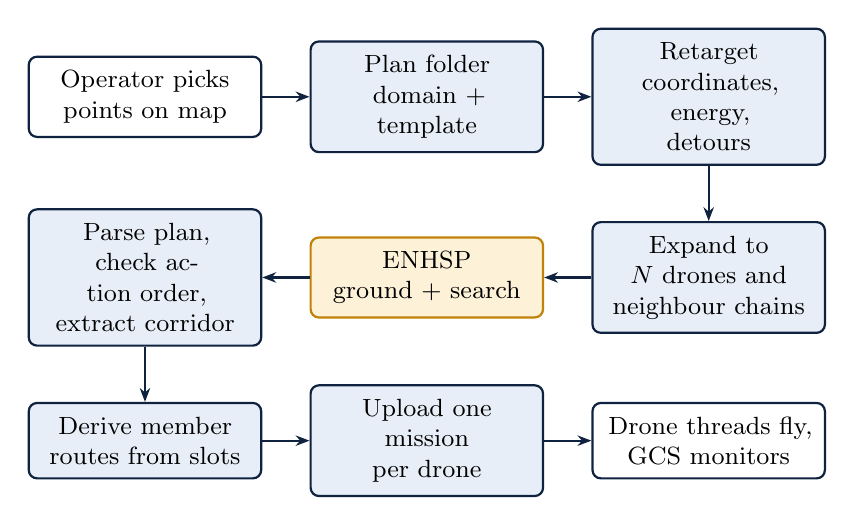
\begin{tikzpicture}[node distance=7mm and 6mm]
  \node[gbox,text width=2.6cm] (gui) {Operator picks\\points on map};
  \node[box,right=of gui,text width=2.6cm] (tpl) {Plan folder\\domain + template};
  \node[box,right=of tpl,text width=2.6cm] (ret) {Retarget\\coordinates, energy,\\detours};
  \node[box,below=of ret,text width=2.6cm] (exp) {Expand to\\$N$ drones and\\neighbour chains};
  \node[abox,left=of exp,text width=2.6cm] (enhsp) {ENHSP\\ground + search};
  \node[box,left=of enhsp,text width=2.6cm] (chk) {Parse plan,\\check action order,\\extract corridor};
  \node[box,below=of chk,text width=2.6cm] (der) {Derive member\\routes from slots};
  \node[box,right=of der,text width=2.6cm] (up) {Upload one mission\\per drone};
  \node[gbox,right=of up,text width=2.6cm] (fly) {Drone threads fly,\\GCS monitors};
  \draw[arr] (gui)--(tpl);
  \draw[arr] (tpl)--(ret);
  \draw[arr] (ret)--(exp);
  \draw[arr] (exp)--(enhsp);
  \draw[arr] (enhsp)--(chk);
  \draw[arr] (chk)--(der);
  \draw[arr] (der)--(up);
  \draw[arr] (up)--(fly);
\end{tikzpicture}
\end{adjustbox}
\caption[Planning pipeline]{The planning pipeline, from the operator's map input to the drones' flight.}
\label{fig:pipeline}
\end{figure}

\section{Plan Kinds and Folders}
The plan service decides how to treat a plan from the \emph{domain name} written inside
\code{domain.pddl}, not from the folder name. This lets a folder be renamed freely and makes the
domain file the single source of truth. Table~\ref{tab:inventory} lists all ten plans.

\begin{table}[H]
\caption[Mission inventory]{Inventory of the ten mission plans}\label{tab:inventory}
\small
\begin{tabularx}{\textwidth}{@{}P{0.21\textwidth}P{0.33\textwidth}Y@{}}
\toprule \textbf{Mission} & \textbf{Folder in plans/} & \textbf{Swarm size} \\ \midrule
Travel & \code{travell} & One or more \\
Search & \code{Search} & At least two \\
V formation & \code{vformation} & Odd count, at least three \\
Grid & \code{gridformation} & At least four \\
Cube & \code{3dgridformation} & At least eight \\
Parabola & \code{parabolaformation} & Exactly three active \\
Figure-eight & \code{figure8formation} & Two up to path capacity \\
Star & \code{starformation} & Six to forty \\
Planets & \code{planets} & Two to eight \\
Inspection & \code{Inspect} & One \\
\bottomrule\end{tabularx}
\end{table}

\section{Run Records}
Every planning request writes a time-stamped folder under \code{plans/<name>/runs/} containing
the exact problem that was solved and the full ENHSP output. These records made it possible to
trace every unsolvable request back to its input, and they are the source of the statistics in
Chapter~\ref{ch:results}.

%% =====================================================================
%%  CHAPTER 4  PDDL MODELLING APPROACH
%% =====================================================================
\chapter{PDDL Modelling Approach}\label{ch:model}

\section{A Shared Vocabulary}
The plans share names for basic drone states. A \textbf{predicate} is a true or
false fact: \code{(gps-ok ?d)} means that drone \code{?d} has a GPS fix.
A \textbf{numeric function} stores a value: \code{(battery ?d)} is the drone's
remaining planning charge. The symbol \code{?d} is a placeholder for a particular
drone; \code{?l} is a location. An action checks these facts before it runs and
updates them afterwards. Table~\ref{tab:vocab} groups the common symbols by purpose.
They are model states, rather than network commands; the run-time commands are
explained separately in Chapter~\ref{ch:comm}.

\begin{table}[H]
\caption[Shared PDDL vocabulary]{Shared predicates and numeric functions used across the domains}\label{tab:vocab}
\small
\begin{tabularx}{\textwidth}{@{}P{0.52\textwidth}Y@{}}
\toprule \textbf{Symbol} & \textbf{Simple meaning} \\ \midrule
\cmd{(at ?d ?l)} & The drone is at this location. \\
\cmd{(landed ?d)} & The drone is on the ground. \\
\cmd{(airborne ?d)} & The drone has taken off. \\
\cmd{(at-cruise-altitude ?d)} & The drone has reached its assigned height. \\
\cmd{(safe-route ?a ?b)} & This route leg is allowed by the model. \\
\cmd{(gps-ok ?d)} & The drone has a usable position fix. \\
\cmd{(communication-ok ?d)} & Its link to the ground controller is assumed working. \\
\cmd{(neighbor-comm-ok ?d)} & Its required formation links are assumed working. \\
\cmd{(drone-healthy ?d)} & The drone passes the model health check. \\
\cmd{(controller-notified ?d)} & A failure notification has been recorded. \\
\cmd{(battery ?d)} & Remaining energy in planning units. \\
\cmd{(minimum-return-battery ?d)} & Energy reserve used by the relevant safety checks. \\
\cmd{(energy-required ?a ?b)} & Energy cost of this route leg. \\
\cmd{(target-altitude ?d)} & The height assigned to this drone. \\
\cmd{(slot-along-offset ?d)} & Its forward or backward offset from the leader. \\
\cmd{(slot-cross-offset ?d)} & Its sideways offset from the leader. \\
\bottomrule\end{tabularx}
\end{table}

\section{The Common Mission Life Cycle}
Every formation begins with pre-flight checks at the source. Each drone must
have working GPS and communication, acceptable health and enough battery.
It takes off, climbs to its assigned cruise height and occupies its slot.
The formation is established only when all required members are ready.

The leader then follows one route leg. A formation-specific close-up or hold
action restores member positions and closes the formation before the next leg.
This repeats until the destination or mission-specific final phase is reached.
Figure~\ref{fig:lifecycle} shows this order; Chapter~\ref{ch:plans} explains the
extra rules for individual missions.

\begin{figure}[H]
\centering
\begin{adjustbox}{max width=\linewidth}
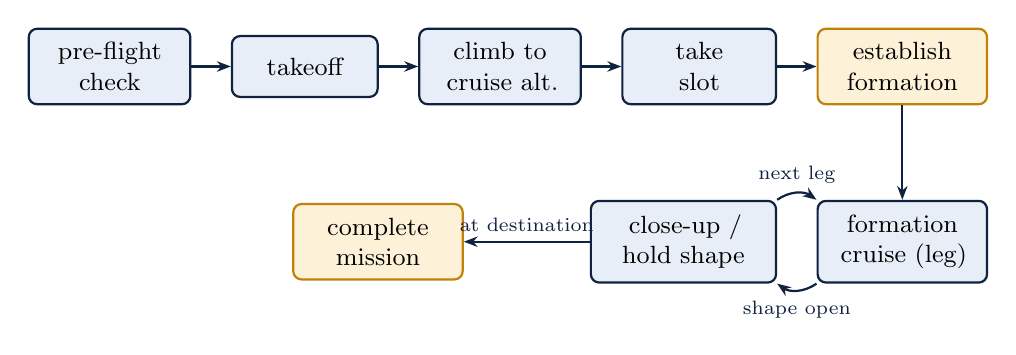
\begin{tikzpicture}[node distance=5mm and 5mm, every node/.style={font=\footnotesize}]
  \node[box,text width=1.7cm] (pf) {pre-flight\\check};
  \node[box,right=of pf,text width=1.5cm] (to) {takeoff};
  \node[box,right=of to,text width=1.7cm] (cl) {climb to\\cruise alt.};
  \node[box,right=of cl,text width=1.6cm] (sl) {take\\slot};
  \node[abox,right=of sl,text width=1.8cm] (es) {establish\\formation};
  \node[box,below=12mm of es,text width=1.8cm] (cr) {formation\\cruise (leg)};
  \node[box,left=of cr,text width=2.0cm] (cu) {close-up /\\hold shape};
  \node[abox,left=16mm of cu,text width=1.8cm] (cm) {complete\\mission};
  \draw[arr] (pf)--(to); \draw[arr] (to)--(cl); \draw[arr] (cl)--(sl); \draw[arr] (sl)--(es);
  \draw[arr] (es)--(cr);
  \draw[arr] (cr.south west) to[bend left=35] node[below,font=\scriptsize]{shape open} (cu.south east);
  \draw[arr] (cu.north east) to[bend left=35] node[above,font=\scriptsize]{next leg} (cr.north west);
  \draw[arr] (cu)--node[above,font=\scriptsize]{at destination}(cm);
\end{tikzpicture}
\end{adjustbox}
\caption[Common mission life cycle]{The life cycle shared by the formation plans. Each box is one PDDL action (or one
action per drone).}
\label{fig:lifecycle}
\end{figure}

The take-off step itself is short but illustrates the style used throughout:

\begin{lstlisting}
(:action takeoff
    :parameters (?d - drone ?l - location)
    :precondition (and (at ?d ?l) (source ?l) (landed ?d)
                       (preflight-done ?d)
                       (gps-ok ?d) (communication-ok ?d) (drone-healthy ?d))
    :effect (and (not (landed ?d)) (airborne ?d) (flying ?d)
                 (assign (altitude ?d) (hover-altitude ?d))))
\end{lstlisting}

\section{Design Patterns for Tractable Swarm Models}
\paragraph{Plan the leader route}
For a rigid formation, ENHSP chooses the leader's route. The service then builds
the other routes by placing each drone at its assigned offset. This avoids asking
the planner to search separately for every follower's geographic path.

\paragraph{Describe neighbours, check readiness}
Neighbour facts record which drones belong next to each other. Most domains check
a single readiness flag for each drone, rather than testing every link separately.
The parabola domain checks individual directed links as well. A neighbour fact
alone does not send a message or prove that a live radio link is working.

\paragraph{Launch cube layers in order}
A layer is allowed to launch only after the layer below has reached its assigned
height. Named layer states express this order more directly than comparing two
changing counters. The rule reduces difficult search and keeps the launch sequence clear.

\paragraph{Keep template facts complete}
The expansion service copies per-drone facts line by line. Each complete fact
must therefore fit on one source line. Otherwise an added drone may receive an
incomplete initial state, which can make a feasible mission appear unsolvable.

%% =====================================================================
%%  CHAPTER 5  MISSION PLANS
%% =====================================================================
\section{Understanding the ENHSP Result}
ENHSP returns a sequence of grounded actions: each placeholder has been replaced
by a named drone or location. Read the sequence from top to bottom. An action
is possible only when its preconditions hold in the state produced by the
previous actions. Its effects then create the state for the next step.
\begin{itemize}
\item \textbf{Action order} tells the service which mission phases are required.
Leading step values in a sequential plan do not specify actual drone flight duration.
\item \textbf{Plan length} counts symbolic actions. It is not route length or drone count.
\item \textbf{Planning time} measures solving effort, rather than mission flight time.
\item \textbf{Expanded and evaluated states} describe the search effort; they are
not completed flights or success percentages.
\end{itemize}
A returned plan satisfies the written goal under the supplied initial conditions.
It still needs parsing, mission-specific checks and route conversion. If ENHSP
returns no plan, I first check the route, energy and formation inputs, then the
solver's error, timeout or memory messages. A timeout does not prove the goal
impossible. The next chapter shows a short travel result and explains the
mission-specific facts that make each plan different.

\chapter{The Mission Plans}\label{ch:plans}
This chapter describes each of the ten plans: what the mission does, how it is picked on the map,
the key facts of its model and the ordering of its actions.

\section{Point-to-Point Travel}
\paragraph{Mission}
The whole selected swarm flies one shared route from a picked source to a picked destination,
optionally around a marked no-fly area. The template's single drone \code{drone1} is cloned to
every selected drone.

\paragraph{Model}
This is the base domain, and it contains the richest fault handling (Chapter~\ref{ch:faults}).
Before each move a drone performs \code{check-distance} and \code{check-battery}; if the battery
cannot cover the leg, {\small\code{notify-insufficient-battery}} records the fact instead. A route is
planned only when every safety check passes:

\begin{lstlisting}
(:action plan-safe-route
    :parameters (?d - drone ?from - location ?to - location)
    :precondition (and (at ?d ?from) (connected ?from ?to) (safe-route ?from ?to)
                       (battery-checked ?d)
                       (gps-ok ?d) (communication-ok ?d) (drone-healthy ?d))
    :effect (route-planned ?d))
\end{lstlisting}

\noindent The \code{travel} action moves the drone, sets it flying, decreases its battery by
\code{energy-required} and clears \code{route-planned}, so the checks are repeated for every leg.
A restricted direct route is marked with \code{restricted-route} and has no \code{safe-route}
fact, so the planner must use the detour waypoints. A typical three-drone plan from the run logs
is shown below.

\recordlabel{Illustrative travel output (one drone, one leg)}
\begin{lstlisting}[style=plain]
0.0: (check-distance drone1 source destination)
1.0: (check-battery drone1 source destination)
2.0: (plan-safe-route drone1 source destination)
3.0: (travel drone1 source destination)
4.0: (reach-destination drone1 destination)
\end{lstlisting}
\noindent The leading values identify the order of actions in this sequential
plan; they are not measured flight times. The first two actions check whether
the leg and its energy requirement are acceptable. The route is then approved,
travel changes the drone's model location and battery, and the final action
records arrival. A longer route repeats the necessary leg checks. The meaning of solver statistics and the distinction between symbolic steps
and flight time are explained in the previous chapter.

\paragraph{How the mission progresses}
Each selected drone follows the approved route from source to destination. For each leg, it checks the route and available battery, records movement and finally records arrival. Adding drones repeats these checks for the additional drone objects; it does not introduce a formation slot.

\paragraph{Communication}
Every active drone needs one ground-controller link. This domain declares no drone-to-drone neighbour relation, so its required peer-neighbour count is zero. The shared route does not by itself provide formation spacing or collision avoidance.

\begin{figure}[H]
\centering
\begin{adjustbox}{max width=\linewidth}
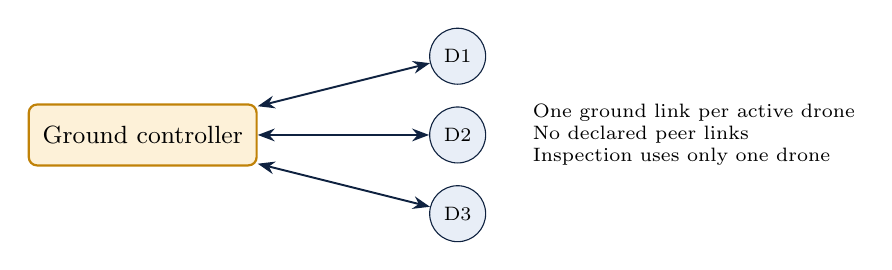
\begin{tikzpicture}[>=Stealth,every node/.style={font=\scriptsize},peer/.style={circle,draw=navy,fill=softblue,minimum size=6mm},conn/.style={<->,navy,line width=0.7pt}]
\node[abox] (g) at (0,0) {Ground controller};
\node[peer] (d0) at (4,1.0) {D1};\draw[conn] (g)--(d0);
\node[peer] (d1) at (4,0.0) {D2};\draw[conn] (g)--(d1);
\node[peer] (d2) at (4,-1.0) {D3};\draw[conn] (g)--(d2);
\node[align=left] at (7,0) {One ground link per active drone\\No declared peer links\\Inspection uses only one drone};
\end{tikzpicture}
\end{adjustbox}
\caption[Travel communication]{Travel communication. Double arrows show required model
relations, not evidence of direct peer packets in the simulator. Every active drone
also needs its ground-controller link.}
\label{fig:comm-travel}
\end{figure}
\subsubsection*{Selected PDDL representation}
\begin{lstlisting}
(communication-ok drone1)
(connected source destination)
(safe-route source destination)
\end{lstlisting}
These initial facts say that drone1 has a controller link and that the direct leg exists and is allowed. The travel action still checks battery and health; a safe-route fact alone is not enough to permit flight.

\paragraph{Completion condition}
Arrival at the destination and mission completion for every selected drone.

\begin{figure}[H]
\centering
% Replace figures/travel_sample.pdf with your simulator screenshot.
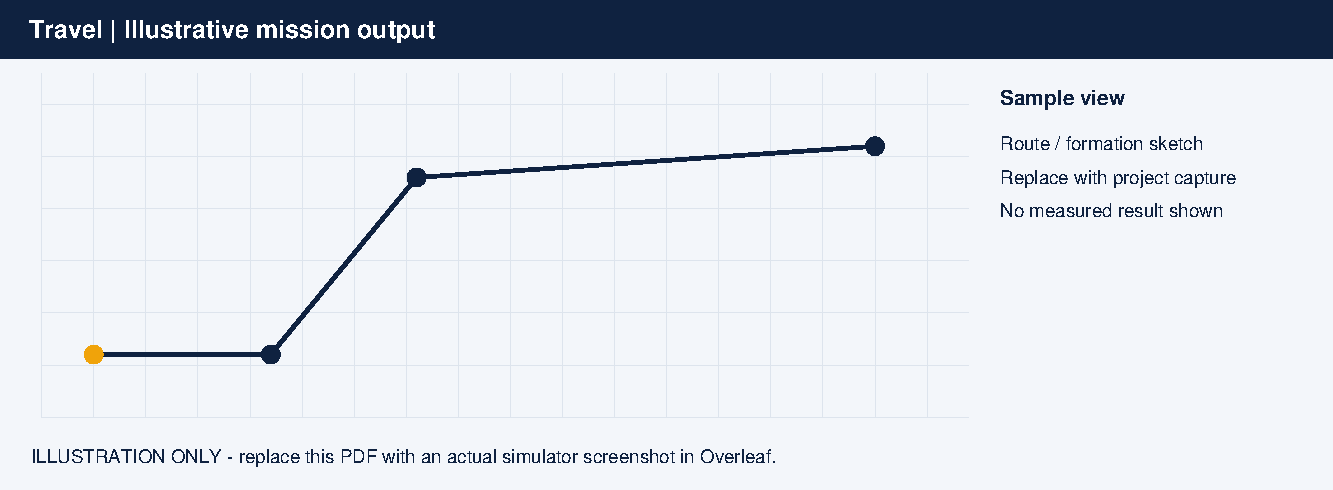
\includegraphics[width=\linewidth]{figures/travel_sample.pdf}
\caption[Travel sample output]{Travel sample output. This schematic is an illustration,
not a recorded simulator result; replace it with the corresponding project screenshot.}
\label{fig:output-travel}
\end{figure}

\section{Forest Area Search}
\paragraph{Mission}
A marked forest polygon is split into lanes, and each drone covers its own lane from a common
base and returns. Unlike travel, each drone has its own route. At least two drones are needed.

\paragraph{Model}
The type \code{forest-area} represents a lane, and \code{(assigned ?d ?a)} gives each drone its
lane. The domain adds an explicit separation check between any two drones, using a pairwise
numeric limit of 10\,m:

\begin{lstlisting}
(:action check-drone-separation
    :parameters (?d1 - drone ?d2 - drone ?l1 - location ?l2 - location)
    :precondition (and (at ?d1 ?l1) (at ?d2 ?l2) (not (= ?d1 ?d2))
                       (>= (distance ?l1 ?l2) (minimum-drone-separation ?d1 ?d2)))
    :effect (and (safe-separation ?d1 ?d2) (separation-ok ?d1) (separation-ok ?d2)))
\end{lstlisting}

\noindent A drone starts its search, moves through its assigned lane and marks
the covered area. After the forest is covered, it returns to base and records
completion. If its battery reaches the return reserve, an emergency-return
action marks the drone as returning.

\paragraph{How the mission progresses}
The selected polygon is divided into search lanes. Each drone leaves the base, visits the points assigned to its lane, marks its area covered and returns to the base. More drones divide the coverage work among more lanes, subject to valid area geometry and sufficient separation.

\paragraph{Communication}
Each drone needs one ground-controller link. There is no declared peer communication topology in this domain: required peer neighbours are zero. Pairwise safe-separation facts describe spacing checks, rather than radio links.

\begin{figure}[H]
\centering
\begin{adjustbox}{max width=\linewidth}
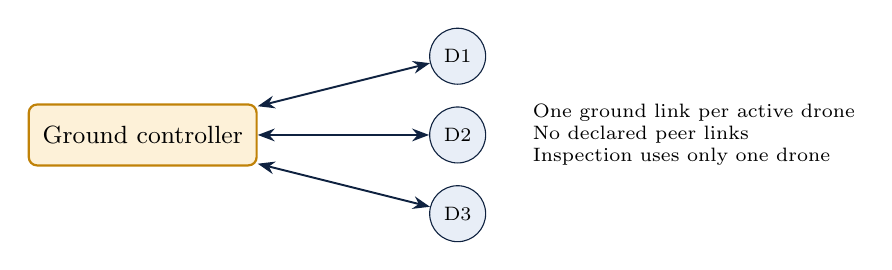
\begin{tikzpicture}[>=Stealth,every node/.style={font=\scriptsize},peer/.style={circle,draw=navy,fill=softblue,minimum size=6mm},conn/.style={<->,navy,line width=0.7pt}]
\node[abox] (g) at (0,0) {Ground controller};
\node[peer] (d0) at (4,1.0) {D1};\draw[conn] (g)--(d0);
\node[peer] (d1) at (4,0.0) {D2};\draw[conn] (g)--(d1);
\node[peer] (d2) at (4,-1.0) {D3};\draw[conn] (g)--(d2);
\node[align=left] at (7,0) {One ground link per active drone\\No declared peer links\\Inspection uses only one drone};
\end{tikzpicture}
\end{adjustbox}
\caption[Search communication]{Search communication. Double arrows show required model
relations, not evidence of direct peer packets in the simulator. Every active drone
also needs its ground-controller link.}
\label{fig:comm-search}
\end{figure}
\subsubsection*{Selected PDDL representation}
\begin{lstlisting}
(assigned drone1 area1)
(assigned drone2 area2)
(communication-ok drone1)
(communication-ok drone2)
\end{lstlisting}
The assignments give the drones different areas. The communication facts represent their controller links. The model checks search progress and separation separately; assigning two lanes does not establish a peer link.

\paragraph{Completion condition}
All assigned areas covered, all drone missions complete and drones back at base.

\begin{figure}[H]
\centering
% Replace figures/search_sample.pdf with your simulator screenshot.
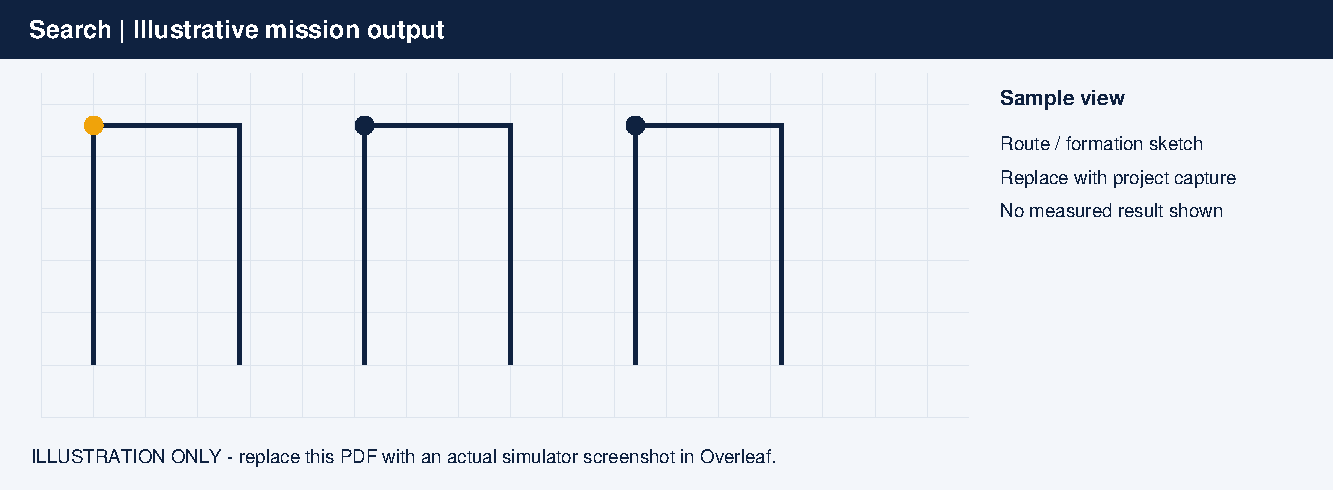
\includegraphics[width=\linewidth]{figures/search_sample.pdf}
\caption[Search sample output]{Search sample output. This schematic is an illustration,
not a recorded simulator result; replace it with the corresponding project screenshot.}
\label{fig:output-search}
\end{figure}

\section{V Formation}
\paragraph{Mission}
Picked like travel. A leader (apex) flies the corridor and the other drones form two wings
behind it. Each rank sits 17.32\,m back and 20\,m to the side of the one before it, so the wing
angle is $60^\circ$ (Figure~\ref{fig:vgrid}a). Extra drones add further ranks.

\paragraph{Model}
Wings launch after a short delay: \code{hold-position} lets the airborne leader wait, increasing
\code{seconds-since-leader-airborne} until it reaches \code{wing-launch-delay}. Each wing drone
takes its slot, and \code{establish-v-formation} requires every wing drone to be in formation,
at the same location, at altitude and with \code{neighbor-comm-ok}. The pairwise fact
\code{(wing-neighbor ?d1 ?d2)} records the chain leader--rank\,1--rank\,2 along each wing; the
expansion code rebuilds this chain correctly for any larger odd drone count.


\paragraph{How the mission progresses}
The leader takes off first and the wing drones launch after the required delay. Each wing drone moves into its assigned slot behind the leader. The leader then follows the route, and the wing positions are restored after each leg so that the V remains ready for the next move.

\paragraph{Communication}
The leader has two wing neighbours, one on either side. An inner wing drone has two neighbours along its own wing; the last drone on a wing has one. In the smallest V, each wing drone talks only to the leader. These are declared model relations; run-time traffic is coordinated through the ground station.

\begin{figure}[H]
\centering
\begin{adjustbox}{max width=\linewidth}
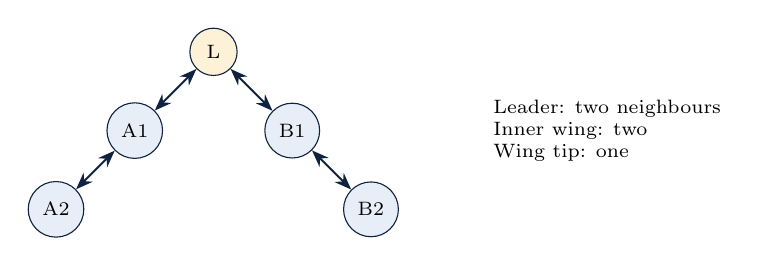
\begin{tikzpicture}[>=Stealth,every node/.style={font=\scriptsize},peer/.style={circle,draw=navy,fill=softblue,minimum size=6mm},conn/.style={<->,navy,line width=0.7pt}]
\node[peer,fill=softamber] (l) at (0,1) {L};\node[peer] (a1) at (-1,0) {A1};\node[peer] (a2) at (-2,-1) {A2};\draw[conn] (l)--(a1);\draw[conn] (a1)--(a2);\node[peer] (b1) at (1,0) {B1};\node[peer] (b2) at (2,-1) {B2};\draw[conn] (l)--(b1);\draw[conn] (b1)--(b2);\node[align=left] at (5,0) {Leader: two neighbours\\Inner wing: two\\Wing tip: one};
\end{tikzpicture}
\end{adjustbox}
\caption[V formation communication]{V formation communication. Double arrows show required model
relations, not evidence of direct peer packets in the simulator. Every active drone
also needs its ground-controller link.}
\label{fig:comm-v}
\end{figure}
\subsubsection*{Selected PDDL representation}
\begin{lstlisting}
(wing-neighbor drone-lead drone-left)
(wing-neighbor drone-left drone-lead)
(neighbor-comm-ok drone-left)
\end{lstlisting}
The two pair facts describe both directions of one wing link. The last fact summarises the left drone's neighbour readiness. Formation actions check readiness flags; they do not establish each pair as a live network connection.

\paragraph{Completion condition}
The full formation reaches the destination and the formation mission is marked complete.

\begin{figure}[H]
\centering
% Replace figures/v_sample.pdf with your simulator screenshot.
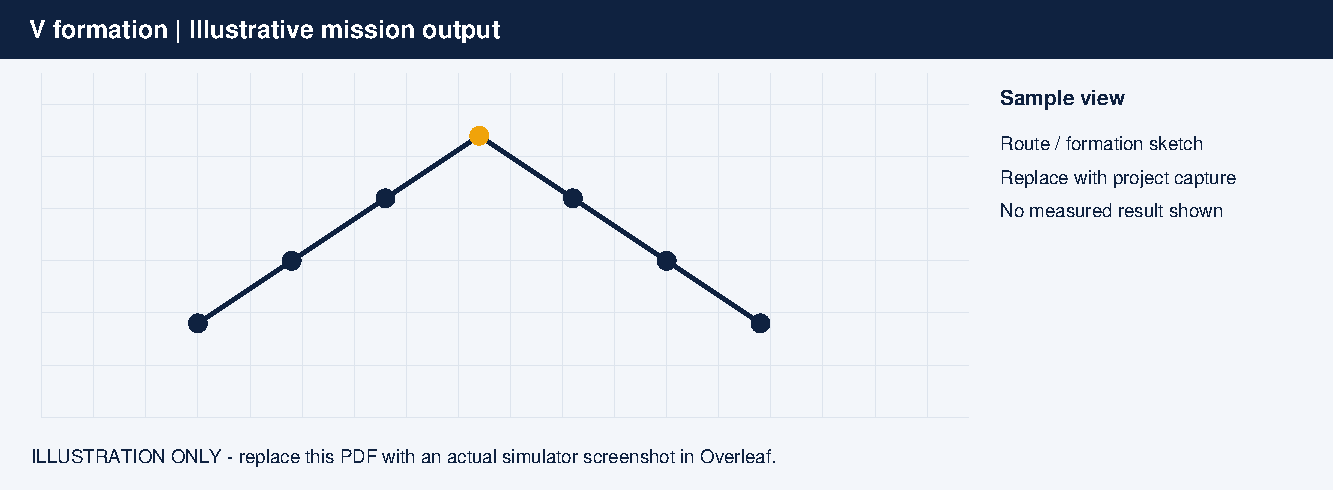
\includegraphics[width=\linewidth]{figures/v_sample.pdf}
\caption[V formation sample output]{V formation sample output. This schematic is an illustration,
not a recorded simulator result; replace it with the corresponding project screenshot.}
\label{fig:output-v}
\end{figure}

\section{Two-Dimensional Grid Formation}
\paragraph{Mission}
The drones fly as a flat grid, 10\,m apart in every direction (Figure~\ref{fig:vgrid}b). A square
count gives a square grid; otherwise the most square rectangle that tiles the count exactly is
used. At least four drones are needed.

\paragraph{Model}
Each drone coordinates only with up to four neighbours (front, back, left, right), recorded by
\code{grid-neighbor}. The leader's corridor is planned, and \code{close-up-grid} restores every
member's cell after each leg. This domain needs ENHSP's naive grounder beyond about a dozen
drones.

\begin{figure}[H]
\centering
\begin{adjustbox}{max width=\linewidth}
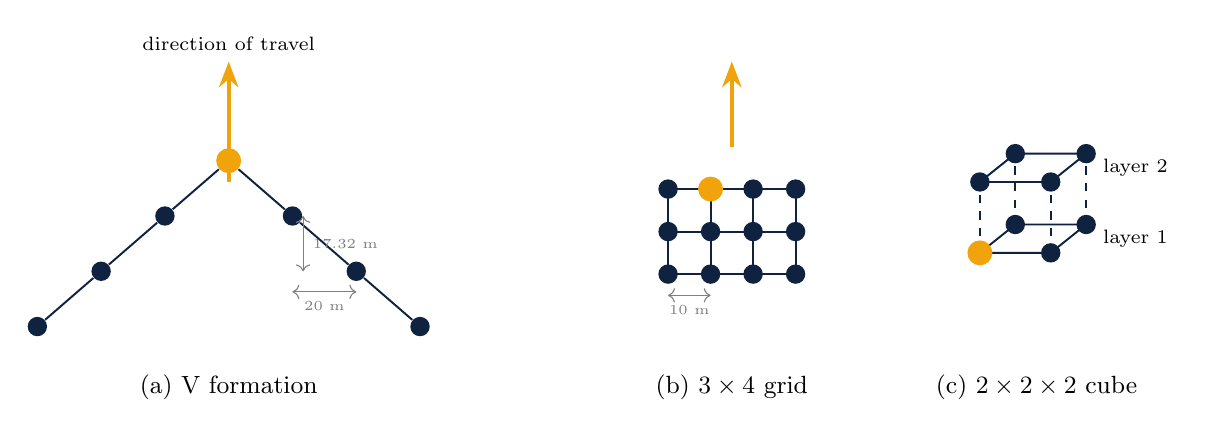
\begin{tikzpicture}[scale=0.9]
  % (a) V formation
  \begin{scope}
    \draw[amber,line width=1.4pt,-{Stealth}] (0,-0.3)--(0,1.4) node[above,font=\scriptsize,black]{direction of travel};
    \node[leader] (L) at (0,0) {};
    \foreach \i in {1,2,3} {
      \node[drone] (l\i) at (-\i*0.9,-\i*0.78) {};
      \node[drone] (r\i) at (\i*0.9,-\i*0.78) {};
    }
    \draw[link] (L)--(l1)--(l2)--(l3); \draw[link] (L)--(r1)--(r2)--(r3);
    \draw[<->,gray,thin] (1.05,-0.78)--(1.05,-1.56) node[midway,right,font=\tiny]{17.32 m};
    \draw[<->,gray,thin] (0.9,-1.85)--(1.8,-1.85) node[midway,below,font=\tiny]{20 m};
    \node[font=\small] at (0,-3.2) {(a) V formation};
  \end{scope}
  % (b) grid
  \begin{scope}[xshift=6.2cm,yshift=-0.4cm]
    \draw[amber,line width=1.4pt,-{Stealth}] (0.9,0.6)--(0.9,1.8);
    \foreach \r in {0,1,2} \foreach \c in {0,1,2,3} {
      \coordinate (g\r\c) at (\c*0.6,-\r*0.6);
    }
    \foreach \r in {0,1,2} { \draw[link] (g\r0)--(g\r3); }
    \foreach \c in {0,1,2,3} { \draw[link] (g0\c)--(g2\c); }
    \foreach \r in {0,1,2} \foreach \c in {0,1,2,3} { \node[drone] at (g\r\c) {}; }
    \node[leader] at (g01) {};
    \draw[<->,gray,thin] (0,-1.5)--(0.6,-1.5) node[midway,below,font=\tiny]{10 m};
    \node[font=\small] at (0.9,-2.8) {(b) $3\times4$ grid};
  \end{scope}
  % (c) cube
  \begin{scope}[xshift=10.6cm,yshift=-1.3cm]
    \foreach \z in {0,1} \foreach \x in {0,1} \foreach \y in {0,1}
      \coordinate (c\x\y\z) at ({\x*1.0+\y*0.5},{\z*1.0+\y*0.4});
    \foreach \z in {0,1} {
      \draw[link] (c00\z)--(c10\z)--(c11\z)--(c01\z)--cycle; }
    \foreach \x in {0,1} \foreach \y in {0,1} { \draw[link,dashed] (c\x\y0)--(c\x\y1); }
    \foreach \z in {0,1} \foreach \x in {0,1} \foreach \y in {0,1} { \node[drone] at (c\x\y\z) {}; }
    \node[leader] at (c000) {};
    \node[font=\scriptsize,right] at (1.6,0.2) {layer 1};
    \node[font=\scriptsize,right] at (1.6,1.2) {layer 2};
    \node[font=\small] at (0.8,-1.9) {(c) $2\times2\times2$ cube};
  \end{scope}
\end{tikzpicture}
\end{adjustbox}
\caption[Rigid formation layouts]{Rigid formations. The amber drone is the leader whose corridor ENHSP plans; lines show
the neighbour links each drone must keep. In the cube, vertical layers are separated by
height.}
\label{fig:vgrid}
\end{figure}


\paragraph{How the mission progresses}
Drones take off, reach a common cruise height and occupy rectangular grid cells. The leader flies the corridor. After a leg, close-up-grid places members at the corresponding cells before the next leg begins. Increasing the swarm rebuilds the rows, columns and neighbour list.

\paragraph{Communication}
A drone inside the grid has four neighbours: front, back, left and right. A boundary drone has fewer: normally three on an edge and two at a corner. A grid with a single row or column has at most two. Diagonal cells are not grid neighbours.

\begin{figure}[H]
\centering
\begin{adjustbox}{max width=\linewidth}
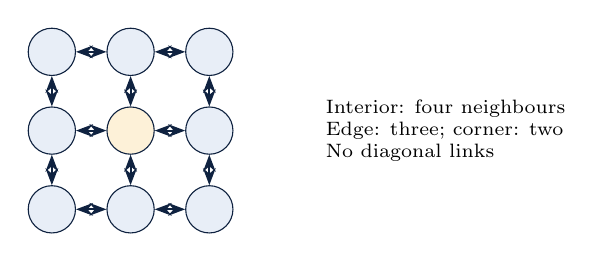
\begin{tikzpicture}[>=Stealth,every node/.style={font=\scriptsize},peer/.style={circle,draw=navy,fill=softblue,minimum size=6mm},conn/.style={<->,navy,line width=0.7pt}]
\node[peer] (g00) at (0,0) {};\node[peer] (g01) at (1,0) {};\draw[conn] (g00)--(g01);\node[peer] (g02) at (2,0) {};\draw[conn] (g01)--(g02);\node[peer] (g10) at (0,-1) {};\draw[conn] (g00)--(g10);\node[peer,fill=softamber] (g11) at (1,-1) {};\draw[conn] (g10)--(g11);\draw[conn] (g01)--(g11);\node[peer] (g12) at (2,-1) {};\draw[conn] (g11)--(g12);\draw[conn] (g02)--(g12);\node[peer] (g20) at (0,-2) {};\draw[conn] (g10)--(g20);\node[peer] (g21) at (1,-2) {};\draw[conn] (g20)--(g21);\draw[conn] (g11)--(g21);\node[peer] (g22) at (2,-2) {};\draw[conn] (g21)--(g22);\draw[conn] (g12)--(g22);\node[align=left] at (5,-1) {Interior: four neighbours\\Edge: three; corner: two\\No diagonal links};
\end{tikzpicture}
\end{adjustbox}
\caption[Grid formation communication]{Grid formation communication. Double arrows show required model
relations, not evidence of direct peer packets in the simulator. Every active drone
also needs its ground-controller link.}
\label{fig:comm-grid}
\end{figure}
\subsubsection*{Selected PDDL representation}
\begin{lstlisting}
(grid-neighbor drone-lead drone-member)
(grid-neighbor drone-member drone-lead)
(neighbor-comm-ok drone-member)
\end{lstlisting}
The pair facts identify adjacent cells in the template. During expansion, the service rebuilds these facts for the selected grid. The readiness flag is the condition checked by the formation actions.

\paragraph{Completion condition}
Every member reaches the destination in the required grid mission state.

\begin{figure}[H]
\centering
% Replace figures/grid_sample.pdf with your simulator screenshot.
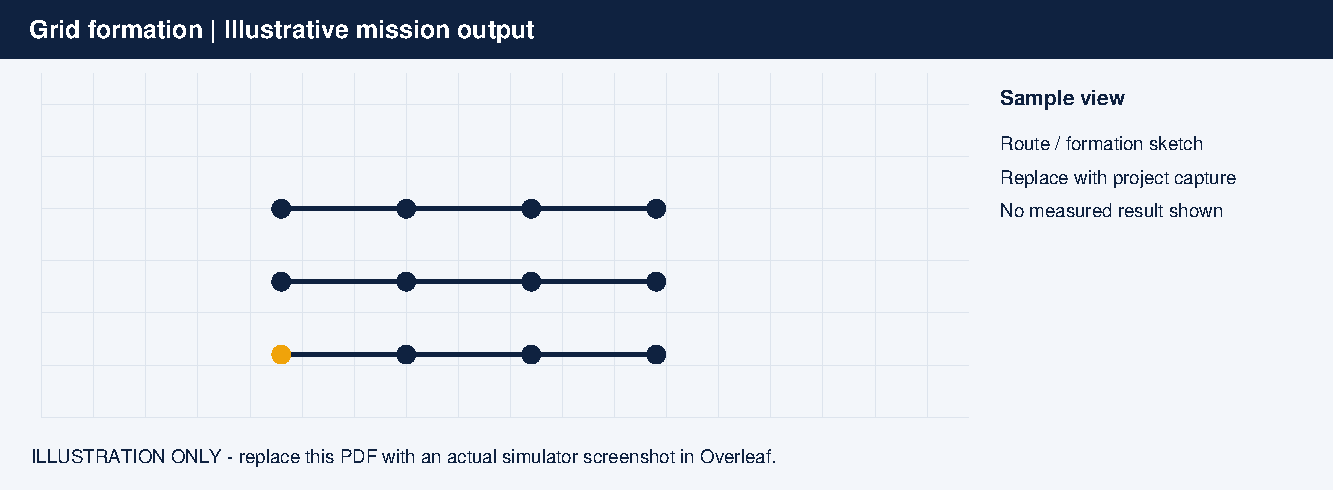
\includegraphics[width=\linewidth]{figures/grid_sample.pdf}
\caption[Grid formation sample output]{Grid formation sample output. This schematic is an illustration,
not a recorded simulator result; replace it with the corresponding project screenshot.}
\label{fig:output-grid}
\end{figure}

\section{Three-Dimensional Cube Formation}
\paragraph{Mission}
The grid extended into the vertical: a solid block of drones flies one corridor, 10\,m apart
horizontally and vertically (Figure~\ref{fig:vgrid}c). A square footprint is chosen and as many
layers as needed are stacked, allowing a partly filled top layer (for example 9 drones become
$3\times2\times2$ with 9 of 12 cells filled; 25 become $3\times3\times3$). At least eight drones
are needed.

\paragraph{Model}
Layers are separated by height, so each drone has its own \code{target-altitude} (base plus
10\,m per layer), and the run-time route adds a per-drone altitude offset. The swarm climbs
layer by layer, bottom first:

\begin{lstlisting}
(:action open-next-layer
    :parameters (?lo - layer ?hi - layer)
    :precondition (and (layer-below ?lo ?hi) (layer-launched ?lo)
                       (not (layer-launched ?hi))
                       (forall (?d - drone)
                           (or (not (in-layer ?d ?lo)) (at-cruise-altitude ?d))))
    :effect (and (layer-launched ?hi)
                 (forall (?d - drone)
                     (when (in-layer ?d ?hi) (cleared-to-launch ?d)))))
\end{lstlisting}

\noindent Each drone may coordinate with up to 24 neighbours: the $3\times3\times3$ block around
it, except itself and the cells directly above and below. Collision avoidance is structural:
fixed spacing, layer-by-layer ascent and a \code{cube-closed} interlock that must hold before
each leg.


\paragraph{How the mission progresses}
Drones are placed in rows, columns and height layers. The lowest layer launches and reaches its height before the next layer is released. Once all occupied cells are ready, the block follows the corridor and restores its shape between legs. A partially filled top layer is allowed.

\paragraph{Communication}
A fully surrounded interior cell has up to 24 declared neighbours: the surrounding cells in a three-by-three-by-three block, excluding itself and the two cells directly above and below. Boundary cells and incomplete layers have fewer. This differs from the four-neighbour flat grid.

\begin{figure}[H]
\centering
\begin{adjustbox}{max width=\linewidth}
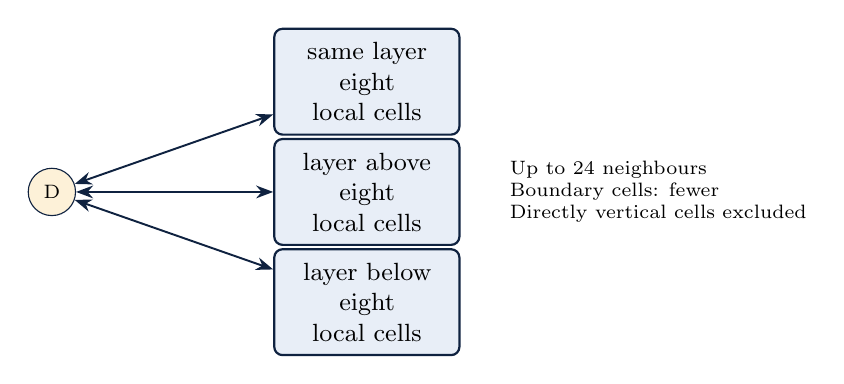
\begin{tikzpicture}[>=Stealth,every node/.style={font=\scriptsize},peer/.style={circle,draw=navy,fill=softblue,minimum size=6mm},conn/.style={<->,navy,line width=0.7pt}]
\node[peer,fill=softamber] (c) at (0,0) {D};\node[box,text width=2.0cm] (l0) at (4,1.4) {same layer\\eight local cells};\draw[conn] (c)--(l0);\node[box,text width=2.0cm] (l1) at (4,0.0) {layer above\\eight local cells};\draw[conn] (c)--(l1);\node[box,text width=2.0cm] (l2) at (4,-1.4) {layer below\\eight local cells};\draw[conn] (c)--(l2);\node[align=left] at (7.7,0) {Up to 24 neighbours\\Boundary cells: fewer\\Directly vertical cells excluded};
\end{tikzpicture}
\end{adjustbox}
\caption[Cube formation communication]{Cube formation communication. Double arrows show required model
relations, not evidence of direct peer packets in the simulator. Every active drone
also needs its ground-controller link.}
\label{fig:comm-cube}
\end{figure}
\subsubsection*{Selected PDDL representation}
\begin{lstlisting}
(cube-neighbor drone-lead drone-member)
(cube-neighbor drone-member drone-lead)
(neighbor-comm-ok drone-member)
\end{lstlisting}
These are selected neighbour facts from the cube template. Expansion rebuilds the actual local cell links. Layer launch conditions and the cube-closed state provide separate ordering rules; the neighbour facts alone do not prevent collisions.

\paragraph{Completion condition}
The occupied cube cells reach the destination with the formation complete.

\begin{figure}[H]
\centering
% Replace figures/cube_sample.pdf with your simulator screenshot.
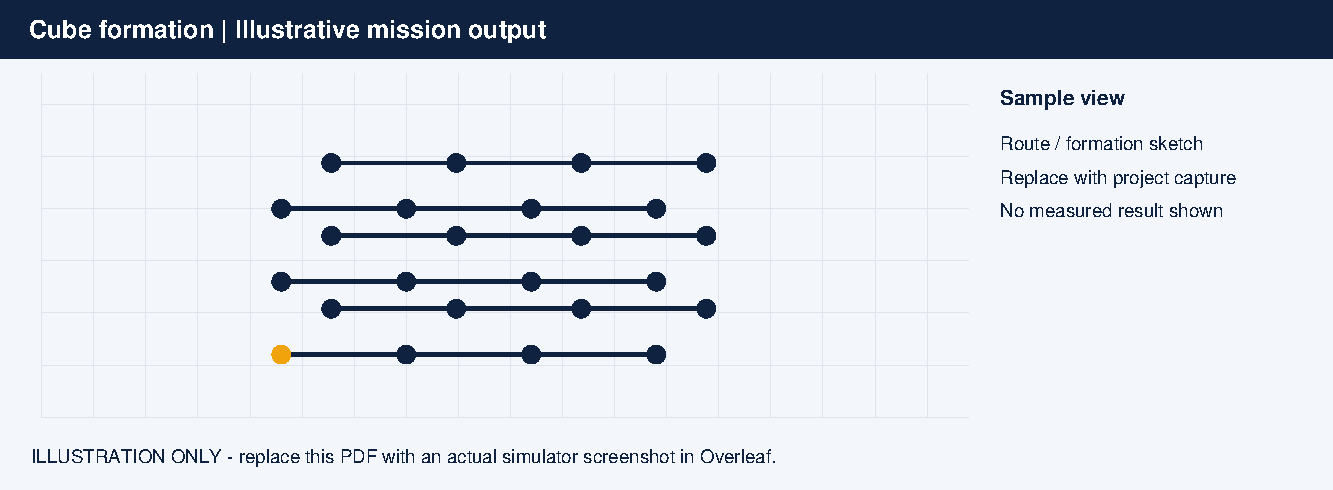
\includegraphics[width=\linewidth]{figures/cube_sample.pdf}
\caption[Cube formation sample output]{Cube formation sample output. This schematic is an illustration,
not a recorded simulator result; replace it with the corresponding project screenshot.}
\label{fig:output-cube}
\end{figure}

\section{Parabola Formation}
\paragraph{Mission}
Three drones fly side by side on one line across the route, 10\,m apart. The middle drone (the
vertex) cruises at 50\,m and the two arm drones at 60\,m, so seen from behind they form an
upward-opening parabola (Figure~\ref{fig:parabola}). Extra selected drones stay on the ground.

\paragraph{Model}
This plan has the most detailed communication model (Section~\ref{sec:paracomm}). Before any
drone may take its slot, every directed link must be established and each drone must confirm
it is in contact with all of its neighbours. The formation action checks the shape: each arm's
target altitude minus the vertex's must equal \code{arm-rise} (10\,m), so a flat line, an
inverted U or lopsided arms give no plan, and every vertex--arm gap (14.14\,m) must be at least
\code{min-separation} (10\,m).

\begin{lstlisting}
(:action establish-parabola-formation
  :parameters (?vtx - drone ?l - location)
  :precondition (and (formation-leader ?vtx) (slot-vertex ?vtx) (in-formation ?vtx)
     (at ?vtx ?l) (at-cruise-altitude ?vtx) (swarm-comm-ready ?vtx)
     (forall (?a - drone)
       (or (not (arm-drone ?a))
           (and (in-formation ?a) (at ?a ?l) (at-cruise-altitude ?a)
                (= (- (target-altitude ?a) (target-altitude ?vtx)) (arm-rise))
                (>= (link-distance ?vtx ?a) (min-separation))
                (swarm-comm-ready ?a)))))
  :effect (and (parabola-established) (formation-at ?l) (shape-held)))
\end{lstlisting}

\begin{figure}[H]
\centering
\begin{adjustbox}{max width=\linewidth}
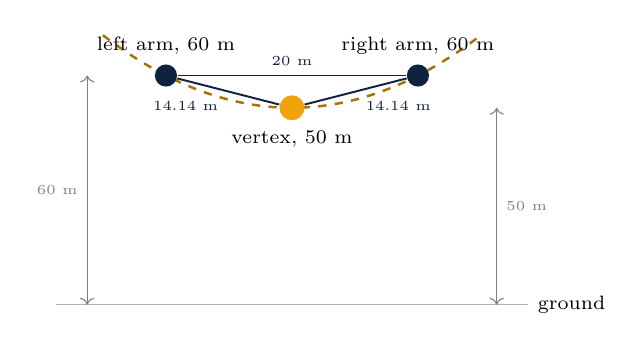
\begin{tikzpicture}[scale=1.0]
  \draw[gray!60] (-3,0)--(3,0) node[right,font=\scriptsize,black]{ground};
  \draw[amber!70!black,dashed,line width=0.9pt,domain=-2.4:2.4,samples=50] plot (\x,{2.5+0.16*\x*\x});
  \node[leader,label={[font=\scriptsize]below:vertex, 50 m}] (v) at (0,2.5) {};
  \node[drone,minimum size=8pt,label={[font=\scriptsize]above:left arm, 60 m}] (a) at (-1.6,2.91) {};
  \node[drone,minimum size=8pt,label={[font=\scriptsize]above:right arm, 60 m}] (b) at (1.6,2.91) {};
  \draw[link] (v)--node[below left,font=\tiny]{14.14 m}(a);
  \draw[link] (v)--node[below right,font=\tiny]{14.14 m}(b);
  \draw[link] (a)--node[above,font=\tiny]{20 m}(b);
  \draw[<->,gray] (2.6,0)--(2.6,2.5) node[midway,right,font=\tiny]{50 m};
  \draw[<->,gray] (-2.6,0)--(-2.6,2.91) node[midway,left,font=\tiny]{60 m};
\end{tikzpicture}
\end{adjustbox}
\caption[Parabola formation]{The parabola formation seen from behind. All three pairs keep a direct link
(full mesh), and every link is within the 100\,m communication range.}
\label{fig:parabola}
\end{figure}

\noindent At run time the vertex corridor is split into legs of at most 200\,m, and the arms are
derived parallel at $\pm10$\,m. All three drones fly one shared timetable, so they arrive at each
waypoint together even though the vertex has 10\,m less to climb.


\paragraph{How the mission progresses}
The vertex drone climbs to its lower assigned height, and the two arm drones climb to their higher heights. Each directed communication link is established, every drone confirms readiness, and only then may drones occupy their slots. The shape is checked before cruise and held again after each leg.

\paragraph{Communication}
Each of the three active drones has two neighbours: the other two drones. Three drone pairs require six directed links because a link in one direction does not automatically create the reverse link. Extra selected drones remain on the ground in this implementation.

\begin{figure}[H]
\centering
\begin{adjustbox}{max width=\linewidth}
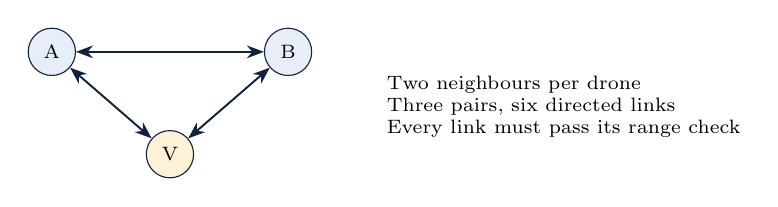
\begin{tikzpicture}[>=Stealth,every node/.style={font=\scriptsize},peer/.style={circle,draw=navy,fill=softblue,minimum size=6mm},conn/.style={<->,navy,line width=0.7pt}]
\node[peer,fill=softamber] (v) at (0,0) {V};\node[peer] (a) at (-1.5,1.3) {A};\node[peer] (b) at (1.5,1.3) {B};\draw[conn] (v)--(a);\draw[conn] (v)--(b);\draw[conn] (a)--(b);\node[align=left] at (5,0.6) {Two neighbours per drone\\Three pairs, six directed links\\Every link must pass its range check};
\end{tikzpicture}
\end{adjustbox}
\caption[Parabola formation communication]{Parabola formation communication. Double arrows show required model
relations, not evidence of direct peer packets in the simulator. Every active drone
also needs its ground-controller link.}
\label{fig:comm-parabola}
\end{figure}
\subsubsection*{Selected PDDL representation}
\begin{lstlisting}
(parabola-neighbor drone-vertex drone-left)
(parabola-neighbor drone-left drone-vertex)
(link-up drone-vertex drone-left)
\end{lstlisting}
The first two facts declare the required pair in both directions. The last fact is an effect produced after establishing one directed link; it is not a substitute for the reverse link. Each link action checks range and radio readiness before setting link-up.

\paragraph{Completion condition}
The three-drone shape reaches the destination and the parabola mission completes.

\begin{figure}[H]
\centering
% Replace figures/parabola_sample.pdf with your simulator screenshot.
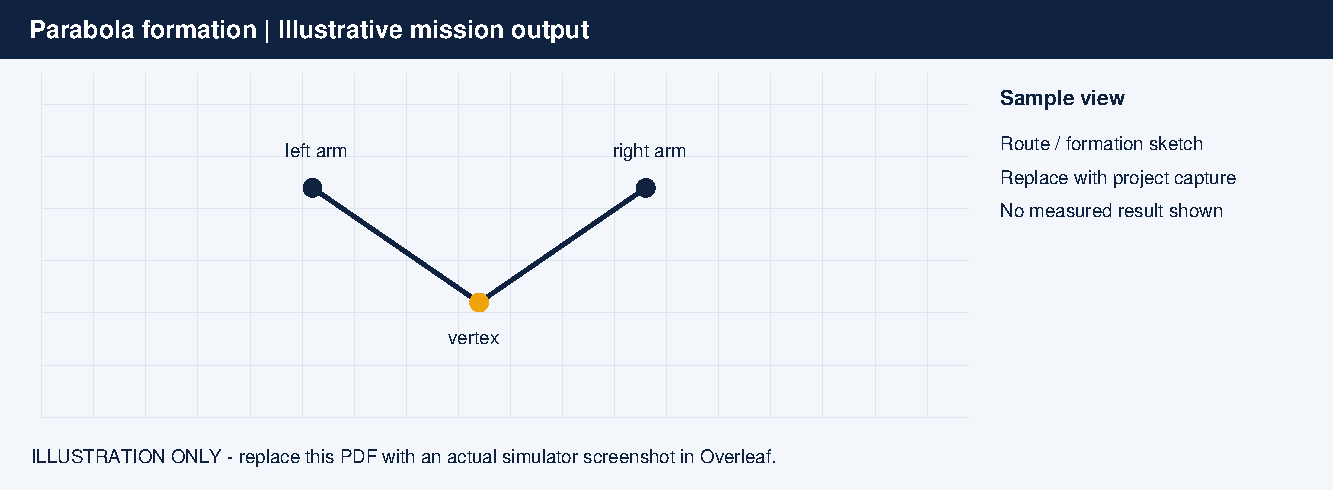
\includegraphics[width=\linewidth]{figures/parabola_sample.pdf}
\caption[Parabola formation sample output]{Parabola formation sample output. This schematic is an illustration,
not a recorded simulator result; replace it with the corresponding project screenshot.}
\label{fig:output-parabola}
\end{figure}

\section{Figure-Eight Train Formation}
\paragraph{Mission}
The swarm flies a figure-eight in the air as a \emph{train}: one drone behind another along the
curve, 10\,m apart. The operator makes four clicks: a base, then the left end, the crossing point
and the right end of the eight. Each lobe is half a lemniscate of Gerono from the crossing to its
clicked end, so the lobes cross at right angles and may differ in size (Figure~\ref{fig:fig8}).
The drones fly from the base to the crossing along a Dubins path (turn radius at least 25\,m),
fly the requested number of laps, and return to their own landing pads.

\paragraph{Model}
Each drone talks only to the drone directly in front and behind (\code{train-neighbor}). The
leader's lap is planned through nine key waypoints with \code{formation-cruise}, and
\code{follow-leader} moves the followers after every leg. Laps are counted numerically:

\begin{lstlisting}
(:action start-next-lap
  :parameters (?lead - drone ?dest - location ?start - location)
  :precondition (and (lap-end ?dest) (lap-start ?start) (figure8-established)
                     (train-closed) (formation-at ?dest) (train-leader ?lead)
                     (at ?lead ?dest) (< (+ (laps-completed) 1) (laps-required)))
  :effect (and (not (formation-at ?dest)) (formation-at ?start)
               (not (at ?lead ?dest)) (at ?lead ?start)
               (increase (laps-completed) 1)))
\end{lstlisting}

\paragraph{Capacity}
The only place the train can meet itself is the crossing. The train length $(N-1)\times10$\,m
plus 14.1\,m of crossing clearance must therefore fit inside the smaller lobe. This rule is
checked in the GUI before planning, again in the plan worker, and inside PDDL itself as a
precondition of \code{establish-figure8-formation}, so ENHSP refuses an over-full eight.

\begin{figure}[H]
\centering
\begin{adjustbox}{max width=\linewidth}
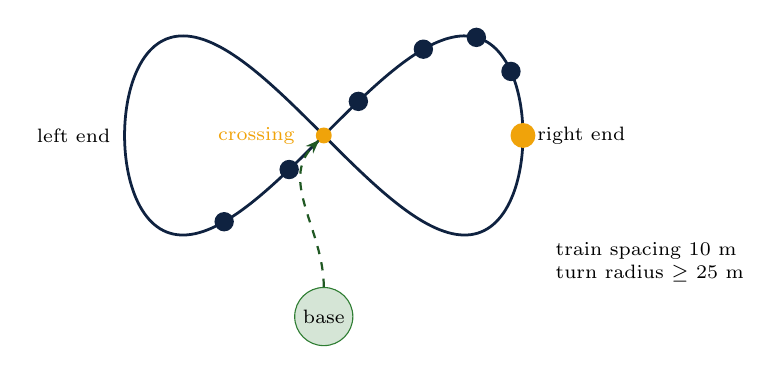
\begin{tikzpicture}[scale=1.15]
  \draw[navy,line width=1.0pt,domain=0:360,samples=120,smooth]
     plot ({2.2*cos(\x)},{1.1*sin(2*\x)});
  \foreach \t in {20,40,60,80,100,120} \node[drone] at ({2.2*cos(\t)},{1.1*sin(2*\t)}) {};
  \node[leader] at ({2.2*cos(0)},{1.1*sin(0)}) {};
  \fill[amber] (0,0) circle (2.5pt) node[left=7pt,font=\scriptsize]{crossing};
  \node[font=\scriptsize,right] at (2.25,0) {right end};
  \node[font=\scriptsize,left] at (-2.25,0) {left end};
  \node[circle,draw=okgreen,fill=okgreen!20,inner sep=2pt,font=\scriptsize] (base) at (0,-2.0) {base};
  \draw[darr,okgreen!70!black] (base) to[out=90,in=-135] (-0.05,-0.05);
  \node[font=\scriptsize,align=left] at (3.6,-1.4) {train spacing 10 m\\turn radius $\geq$ 25 m};
\end{tikzpicture}
\end{adjustbox}
\caption[Figure-eight route]{The figure-eight train. The leader (amber) and followers fly the same path one spacing
apart; the base leg joins the eight tangentially at the crossing.}
\label{fig:fig8}
\end{figure}


\paragraph{How the mission progresses}
The drones join the figure-eight from the base and follow the same curve in order, with a fixed progress gap. The planner records lap progress; the local controller follows the shared pace. After the requested laps, each drone leaves the pattern and returns to its own landing pad.

\paragraph{Communication}
The first and last drones in the ordered train have one neighbour each. Every middle drone has two: the drone immediately ahead and immediately behind. Crossing the same map position does not create an extra neighbour link. The path capacity check limits the total train length.

\begin{figure}[H]
\centering
\begin{adjustbox}{max width=\linewidth}
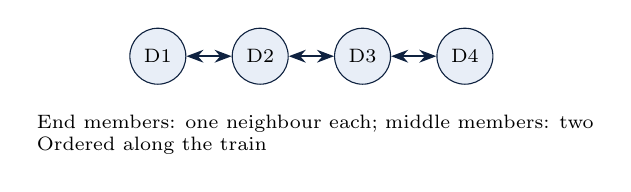
\begin{tikzpicture}[>=Stealth,every node/.style={font=\scriptsize},peer/.style={circle,draw=navy,fill=softblue,minimum size=6mm},conn/.style={<->,navy,line width=0.7pt}]
\node[peer] (c0) at (0.0,0) {D1};\node[peer] (c1) at (1.3,0) {D2};\draw[conn] (c0)--(c1);\node[peer] (c2) at (2.6,0) {D3};\draw[conn] (c1)--(c2);\node[peer] (c3) at (3.9000000000000004,0) {D4};\draw[conn] (c2)--(c3);\node[align=left] at (2,-1) {End members: one neighbour each; middle members: two\\Ordered along the train};
\end{tikzpicture}
\end{adjustbox}
\caption[Figure-eight train communication]{Figure-eight train communication. Double arrows show required model
relations, not evidence of direct peer packets in the simulator. Every active drone
also needs its ground-controller link.}
\label{fig:comm-figure8}
\end{figure}
\subsubsection*{Selected PDDL representation}
\begin{lstlisting}
(train-neighbor drone-lead drone-f1)
(train-neighbor drone-f1 drone-lead)
(neighbor-comm-ok drone-f1)
\end{lstlisting}
These facts describe consecutive train members, rather than all drones close to the crossing. The readiness flag permits formation actions. A shared run-time pace is supplied separately and is not a PDDL message exchange.

\paragraph{Completion condition}
The required laps finish and the drones return to their assigned landing pads.

\begin{figure}[H]
\centering
% Replace figures/figure8_sample.pdf with your simulator screenshot.
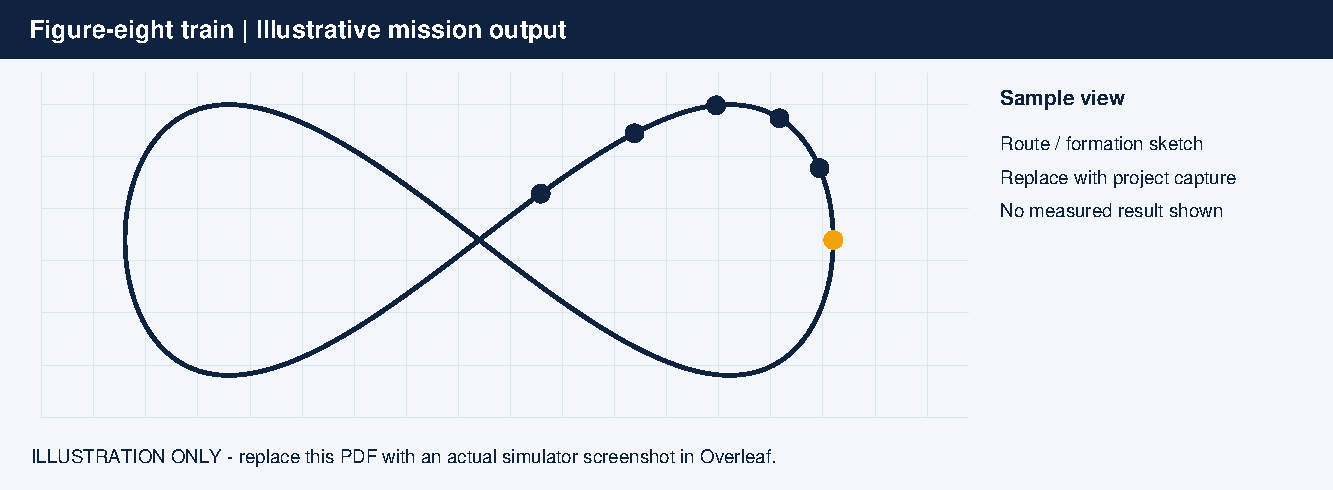
\includegraphics[width=\linewidth]{figures/figure8_sample.pdf}
\caption[Figure-eight train sample output]{Figure-eight train sample output. This schematic is an illustration,
not a recorded simulator result; replace it with the corresponding project screenshot.}
\label{fig:output-figure8}
\end{figure}

\section{Star Drone Show}
\paragraph{Mission}
A stationary show around one picked point. The drones take off from pads in rings, spread into a
circle, and then, for each lap, form a star, return to the circle, spin the circle once, form the
star again, spin the star and return to the circle, before landing on their own pads
(Figure~\ref{fig:shows}a). Six or seven drones make a 3-pointed star, eight or nine a 4-pointed
star, and ten or more a 5-pointed star; 6 to 40 drones are allowed.

\paragraph{Model}
ENHSP sequences \code{form-circle}, then per lap \code{form-star}, \code{form-circle-in-lap},
\code{spin-circle}, \code{form-star-again}, \code{spin-star} and \code{close-lap}, and finally
\code{land-show}. The plan worker checks that exactly this sequence is returned. Every drone keeps
the same order round the centre in the circle and the star, so shape changes never cross paths;
the show is sized until all drones are at least 10\,m apart in each shape and at least 9\,m apart
during transitions.


\paragraph{How the mission progresses}
The drones rise from their pads and spread into a circle. For each lap, they form a star, return to a circle, rotate, form the star again and rotate it. Their order around the centre stays the same through the changes. After all phases, they return and land on their own pads.

\paragraph{Communication}
Each drone has two ring neighbours, the preceding and following drone in cyclic order. The first and last entries are also linked, closing the ring. This relation remains meaningful when the visible shape changes from circle to star. All drones also receive the shared show clock through the ground station.

\begin{figure}[H]
\centering
\begin{adjustbox}{max width=\linewidth}
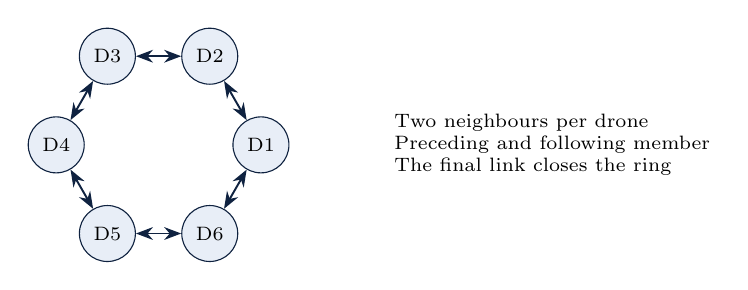
\begin{tikzpicture}[>=Stealth,every node/.style={font=\scriptsize},peer/.style={circle,draw=navy,fill=softblue,minimum size=6mm},conn/.style={<->,navy,line width=0.7pt}]
\node[peer] (r0) at (0:1.3) {D1};\node[peer] (r1) at (60:1.3) {D2};\node[peer] (r2) at (120:1.3) {D3};\node[peer] (r3) at (180:1.3) {D4};\node[peer] (r4) at (240:1.3) {D5};\node[peer] (r5) at (300:1.3) {D6};\draw[conn] (r0)--(r1);\draw[conn] (r1)--(r2);\draw[conn] (r2)--(r3);\draw[conn] (r3)--(r4);\draw[conn] (r4)--(r5);\draw[conn] (r5)--(r0);\node[align=left] at (5,0) {Two neighbours per drone\\Preceding and following member\\The final link closes the ring};
\end{tikzpicture}
\end{adjustbox}
\caption[Star show communication]{Star show communication. Double arrows show required model
relations, not evidence of direct peer packets in the simulator. Every active drone
also needs its ground-controller link.}
\label{fig:comm-star}
\end{figure}
\subsubsection*{Selected PDDL representation}
\begin{lstlisting}
(ring-neighbor drone-lead drone-m1)
(ring-neighbor drone-m1 drone-lead)
(neighbor-comm-ok drone-m1)
\end{lstlisting}
The pair facts are part of the cyclic ordering; expansion creates the complete ring for the selected swarm. The readiness flag is checked when forming the initial circle. Later show phases follow the planned phase order and shared schedule.

\paragraph{Completion condition}
The requested show laps finish and every participating drone lands at the source.

\begin{figure}[H]
\centering
% Replace figures/star_sample.pdf with your simulator screenshot.
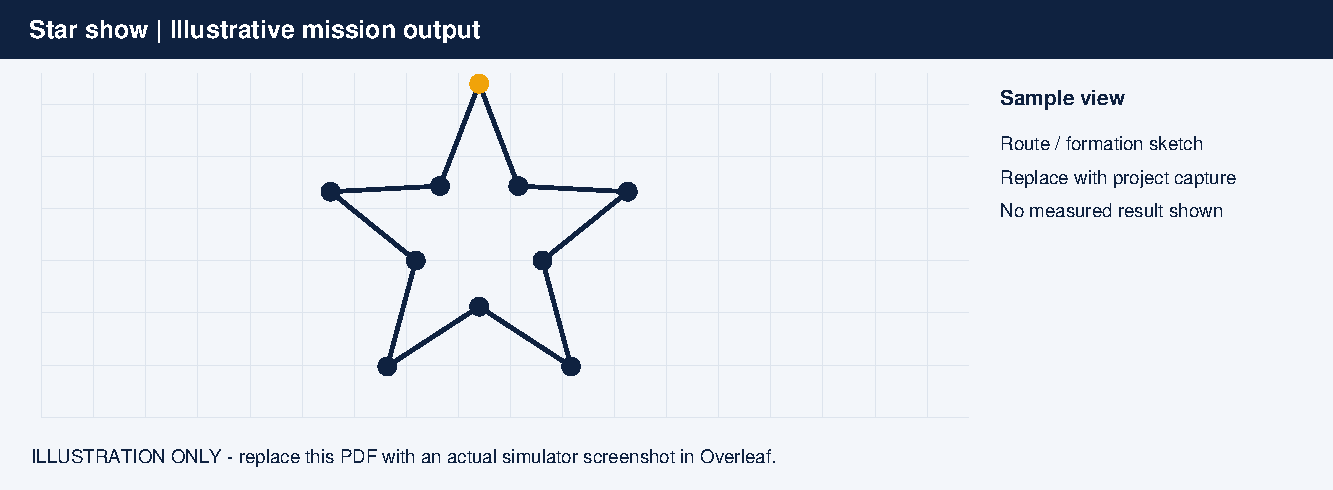
\includegraphics[width=\linewidth]{figures/star_sample.pdf}
\caption[Star show sample output]{Star show sample output. This schematic is an illustration,
not a recorded simulator result; replace it with the corresponding project screenshot.}
\label{fig:output-star}
\end{figure}

\section{Planetary Orbit Show}
\paragraph{Mission}
A solar-system show round one picked point (the sun), with 2 to 8 drones, one per planet. Drone
$k$ orbits at a radius of $50(k+1)$\,m, and neighbouring orbits turn in opposite directions
(Figure~\ref{fig:shows}b). One lap is one turn of the outermost drone; inner drones make as many
whole turns as fit, so all drones line up again on the north line at the end of every lap.

\paragraph{Model}
\code{enter-orbits} may fire only when every drone has climbed and has \code{neighbor-comm-ok},
and only if every pair of orbit neighbours turns in opposite directions:

\begin{lstlisting}
(forall (?a - drone ?b - drone)
    (or (not (orbit-neighbor ?a ?b))
        (and (orbits-clockwise ?a) (orbits-anticlockwise ?b))
        (and (orbits-anticlockwise ?a) (orbits-clockwise ?b))))
\end{lstlisting}

\noindent One \code{fly-lap} follows per lap, counted by \code{laps-completed}, then
\code{land-planets}.

\begin{figure}[H]
\centering
\begin{adjustbox}{max width=\linewidth}
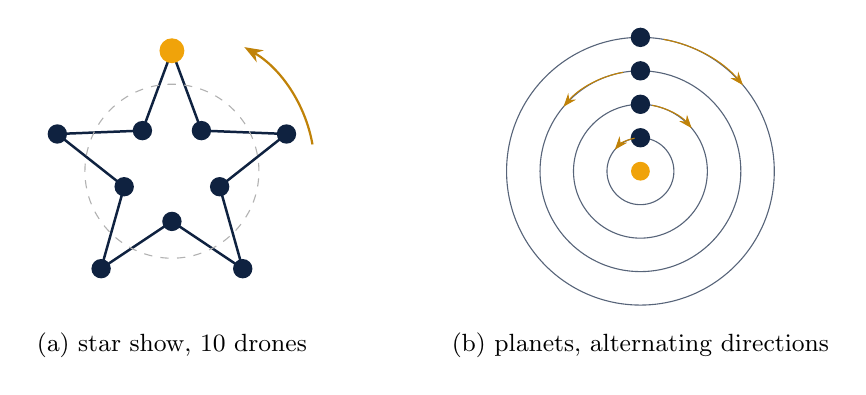
\begin{tikzpicture}[scale=0.85]
  \begin{scope}
    \foreach \k in {0,...,9} {
      \pgfmathsetmacro{\r}{ifthenelse(mod(\k,2)==0,1.8,0.75)}
      \coordinate (s\k) at ({90+\k*36}:\r);
    }
    \draw[navy,line width=0.9pt] (s0)--(s1)--(s2)--(s3)--(s4)--(s5)--(s6)--(s7)--(s8)--(s9)--cycle;
    \draw[gray!60,dashed] (0,0) circle (1.3);
    \foreach \k in {0,...,9} \node[drone] at (s\k) {};
    \node[leader] at (s0) {};
    \draw[amber!80!black,-{Stealth},line width=0.8pt] (2.1,0.4) arc (10:60:2.1);
    \node[font=\small] at (0,-2.6) {(a) star show, 10 drones};
  \end{scope}
  \begin{scope}[xshift=7cm]
    \fill[amber] (0,0) circle (4pt);
    \foreach \k/\dir in {1/1,2/-1,3/1,4/-1} {
      \draw[navy!70] (0,0) circle (\k*0.5);
      \node[drone] at (90:\k*0.5) {};
      \ifnum\dir=1
        \draw[-{Stealth},amber!80!black] (100:\k*0.5) arc (100:140:\k*0.5);
      \else
        \draw[-{Stealth},amber!80!black] (80:\k*0.5) arc (80:40:\k*0.5);
      \fi
    }
    \node[font=\small] at (0,-2.6) {(b) planets, alternating directions};
  \end{scope}
\end{tikzpicture}
\end{adjustbox}
\caption[Star and planetary shows]{Shape-changing shows. Both are flown against a shared timetable so that every phase
starts and ends together for all drones.}
\label{fig:shows}
\end{figure}


\paragraph{How the mission progresses}
Each drone enters its own circular orbit around the selected centre. Adjacent orbit indices have opposite rotation directions. A shared schedule keeps the show phases aligned; after the required laps, all drones return to their landing pads. Increasing the selected count adds orbits within the supported limit.

\paragraph{Communication}
The innermost and outermost orbit drones each have one neighbour. Every intermediate orbit drone has two: the next smaller and next larger orbit. This is a chain ordered by orbit radius, rather than a complete mesh or a ring. With two drones, both have just one neighbour.

\begin{figure}[H]
\centering
\begin{adjustbox}{max width=\linewidth}
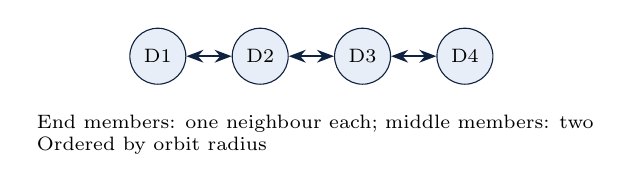
\begin{tikzpicture}[>=Stealth,every node/.style={font=\scriptsize},peer/.style={circle,draw=navy,fill=softblue,minimum size=6mm},conn/.style={<->,navy,line width=0.7pt}]
\node[peer] (c0) at (0.0,0) {D1};\node[peer] (c1) at (1.3,0) {D2};\draw[conn] (c0)--(c1);\node[peer] (c2) at (2.6,0) {D3};\draw[conn] (c1)--(c2);\node[peer] (c3) at (3.9000000000000004,0) {D4};\draw[conn] (c2)--(c3);\node[align=left] at (2,-1) {End members: one neighbour each; middle members: two\\Ordered by orbit radius};
\end{tikzpicture}
\end{adjustbox}
\caption[Planetary show communication]{Planetary show communication. Double arrows show required model
relations, not evidence of direct peer packets in the simulator. Every active drone
also needs its ground-controller link.}
\label{fig:comm-planets}
\end{figure}
\subsubsection*{Selected PDDL representation}
\begin{lstlisting}
(orbit-neighbor drone-mercury drone-venus)
(orbit-neighbor drone-venus drone-mercury)
(orbits-clockwise drone-mercury)
(orbits-anticlockwise drone-venus)
\end{lstlisting}
The orbit pair requires opposite directions before enter-orbits is allowed. When more drones are selected, the service adds adjacent-orbit pairs and alternates their directions. Controller communication and neighbour readiness are checked separately.

\paragraph{Completion condition}
All required laps finish and the participating drones land back at the source.

\begin{figure}[H]
\centering
% Replace figures/planets_sample.pdf with your simulator screenshot.
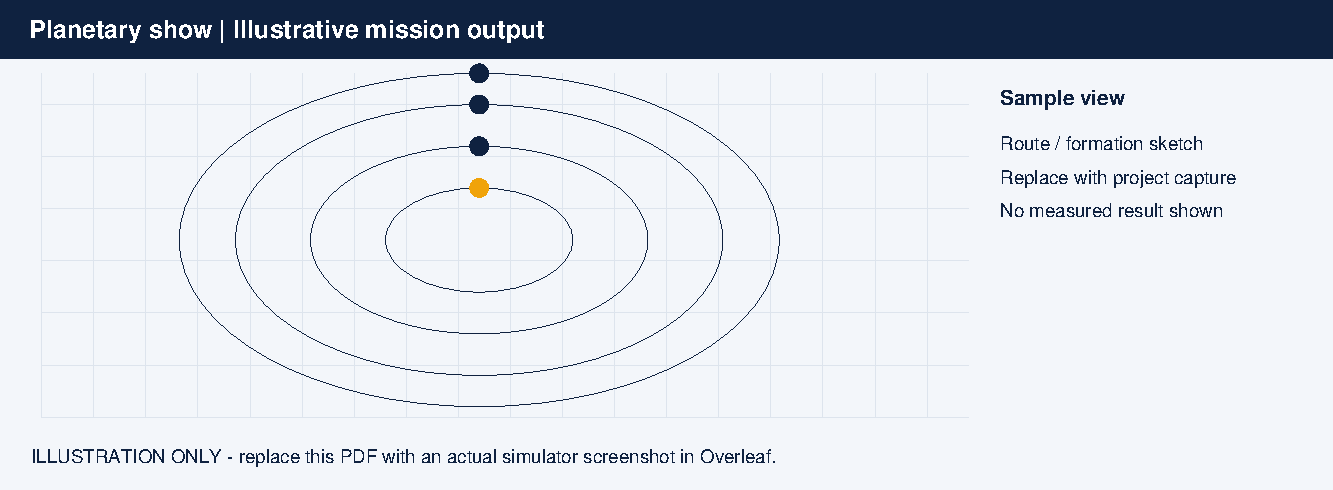
\includegraphics[width=\linewidth]{figures/planets_sample.pdf}
\caption[Planetary show sample output]{Planetary show sample output. This schematic is an illustration,
not a recorded simulator result; replace it with the corresponding project screenshot.}
\label{fig:output-planets}
\end{figure}

\section{Road Inspection}
\paragraph{Mission}
The operator clicks a source and a destination on a road. One drone takes off at the source,
follows the road's exact path to the destination, flies the same road back and lands at the
source. The road geometry comes from an OSRM routing server on OpenStreetMap
data.

\paragraph{Model}
The road is split into at most 12 segments, each with its own length and energy. ENHSP plans
\code{inspect-segment} for each in order, \code{finish-inspection} at the destination,
\code{return-along-road} back segment by segment, and \code{land-at-source}. Each segment
inspection checks GPS, communication, health and that the battery covers the segment. If no road
route exists, a click is more than 30\,m from any road, or the two points are less than 20\,m
apart along the road, the plan fails before anything flies.


\paragraph{How the mission progresses}
The road route is obtained from the selected source and destination and divided into ordered segments. The drone inspects each outbound segment, records that the road is inspected, follows the road back and lands at the source. It follows the road geometry rather than a straight line between the clicks.

\paragraph{Communication}
There is one active inspection drone and one ground-controller link. Its required peer-neighbour count is zero because no second inspection drone or formation relation is created. Supporting a swarm inspection mission would require additional assignment and coordination rules.

\begin{figure}[H]
\centering
\begin{adjustbox}{max width=\linewidth}
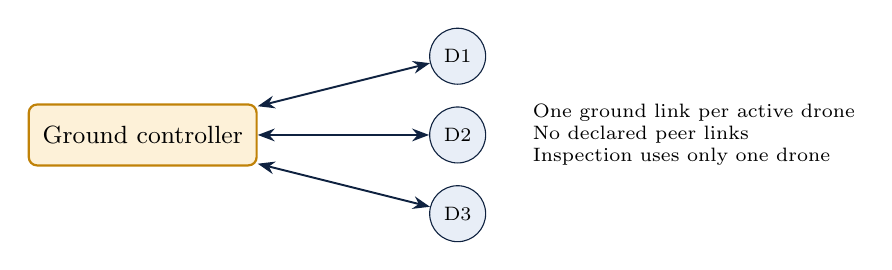
\begin{tikzpicture}[>=Stealth,every node/.style={font=\scriptsize},peer/.style={circle,draw=navy,fill=softblue,minimum size=6mm},conn/.style={<->,navy,line width=0.7pt}]
\node[abox] (g) at (0,0) {Ground controller};
\node[peer] (d0) at (4,1.0) {D1};\draw[conn] (g)--(d0);
\node[peer] (d1) at (4,0.0) {D2};\draw[conn] (g)--(d1);
\node[peer] (d2) at (4,-1.0) {D3};\draw[conn] (g)--(d2);
\node[align=left] at (7,0) {One ground link per active drone\\No declared peer links\\Inspection uses only one drone};
\end{tikzpicture}
\end{adjustbox}
\caption[Road inspection communication]{Road inspection communication. Double arrows show required model
relations, not evidence of direct peer packets in the simulator. Every active drone
also needs its ground-controller link.}
\label{fig:comm-inspect}
\end{figure}
\subsubsection*{Selected PDDL representation}
\begin{lstlisting}
(road-inspected)
(at drone1 source)
(landed drone1)
(mission-completed drone1)
\end{lstlisting}
These selected goal facts explain why reaching the far end alone is insufficient: the road must be inspected and the drone must return and land. The inspect-segment action separately checks the controller link and energy before each segment.

\paragraph{Completion condition}
The road is inspected and the drone returns and lands at the source.

\begin{figure}[H]
\centering
% Replace figures/inspect_sample.pdf with your simulator screenshot.
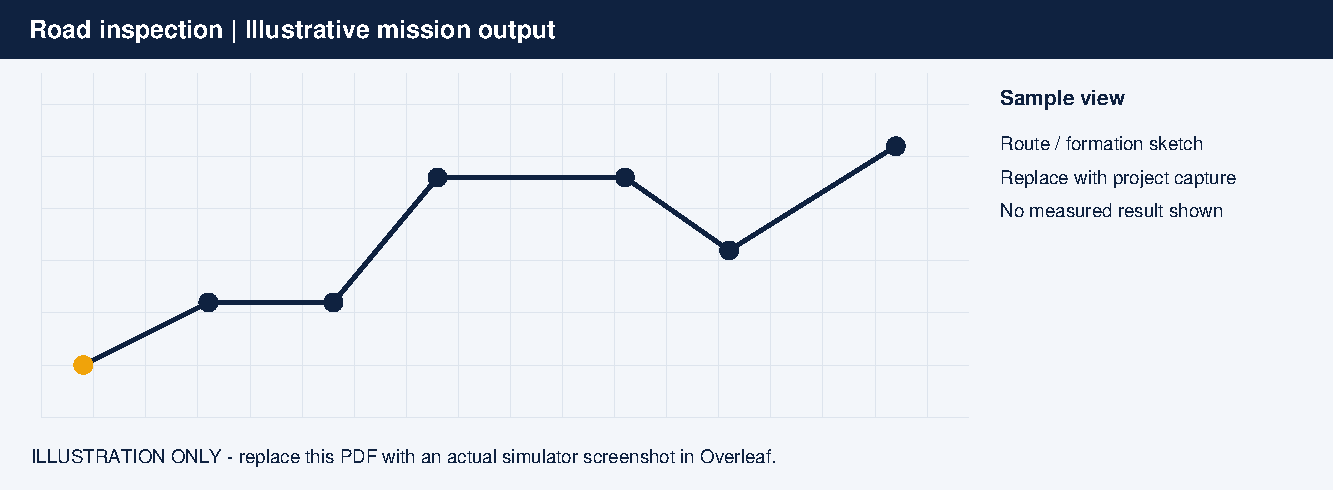
\includegraphics[width=\linewidth]{figures/inspect_sample.pdf}
\caption[Road inspection sample output]{Road inspection sample output. This schematic is an illustration,
not a recorded simulator result; replace it with the corresponding project screenshot.}
\label{fig:output-inspect}
\end{figure}

\section{Swarm Size and Adaptability}
Selecting more drones rebuilds the expandable mission's objects, slots and
neighbour relations. It does not make every mission unlimited. The limits below
separate implementation constraints from examples already demonstrated in the
source report. A demonstrated size is not a proof that every map at that size
is feasible. Battery, route geometry and available solver memory still matter.
\begin{table}[H]
\caption[Swarm size and mission limits]{Swarm size and mission-specific limits}
\small
\begin{tabularx}{\textwidth}{@{}P{0.20\textwidth}P{0.28\textwidth}Y@{}}
\toprule
\textbf{Mission} & \textbf{Accepted size} & \textbf{Practical interpretation} \\\midrule
Travel & One or more & No fixed upper limit stated; resource dependent. \\
Search & At least two & Lanes depend on polygon geometry and separation. \\
V & Odd count from three & Additional paired wing ranks; examples through seven. \\
Grid & At least four & Rebuilt rectangle; larger cases can exhaust grounding memory. \\
Cube & At least eight & Additional cells and layers; demonstrated through 64. \\
Parabola & Exactly three active & Vertex and two arms; additional drones stay grounded. \\
Figure-eight & Two to path capacity & Smaller lobe limits train length; example capacity 27. \\
Star & Six to forty & Implemented show-size range. \\
Planets & Two to eight & One drone per supported orbit. \\
Inspection & One & Current implementation has no swarm expansion. \\
\bottomrule
\end{tabularx}
\end{table}

\section{Summary of the Plans}
Table~\ref{tab:plansummary} compares the ten plans.

\begin{table}[!htb]
\caption[Mission comparison]{Comparison of the mission plans}\label{tab:plansummary}
\small
\begin{tabularx}{\textwidth}{@{}lP{0.2\textwidth}P{0.22\textwidth}Y@{}}
\toprule
\textbf{Plan} & \textbf{Map input} & \textbf{What ENHSP plans} & \textbf{Special feature} \\
\midrule
Travel     & source, destination, no-fly area & every drone's legs & full controller fault responses \\
Search     & base, forest polygon & one lane per drone & pairwise separation check \\
V          & source, destination, no-fly area & leader corridor & timed wing launch \\
Grid       & as V & leader corridor & 4-neighbour links \\
Cube       & as V & leader corridor & layer-by-layer ascent \\
Parabola   & as V & vertex corridor & range-checked link mesh, shape check \\
Figure-8   & base and three points & leader's lap & capacity rule, laps \\
Star       & one point & show phases & circle/star/spin sequence \\
Planets    & one point & show phases & opposite-direction orbits \\
Inspect    & two points on a road & road segments & OSRM road geometry \\
\bottomrule
\end{tabularx}
\end{table}

%% =====================================================================
%%  CHAPTER 6  COMMUNICATION
%% =====================================================================
\chapter{Inter-Drone Communication}\label{ch:comm}
Communication appears at two levels in the simulator. In the PDDL models it is a set of
conditions: a drone may only act if its links are up. At run time it is a real exchange of
messages between the ground station and the drones. This chapter explains both and how they
relate.

\section{Communication in the PDDL Models}
Two flags carry communication state for every drone:
\begin{itemize}
  \item \code{communication-ok}: the link between the drone and the ground controller works;
  \item \code{neighbor-comm-ok}: the drone's links to its formation neighbours work.
\end{itemize}
Formation establishment and movement actions check the relevant readiness conditions;
exact checks vary by mission and phase. A formation
cannot be established, cruise a leg or close up if any member has lost its neighbour links.
Each plan also declares \emph{who} must talk to whom, using a neighbour relation suited to its
shape (Table~\ref{tab:neighbors}, Figure~\ref{fig:topologies}).

\begin{table}[H]
\caption[Formation neighbour relations]{Neighbour relations declared by each formation}\label{tab:neighbors}
\small
\begin{tabularx}{\textwidth}{@{}l>{\ttfamily\footnotesize}lY@{}}
\toprule
\textbf{Plan} & \textbf{\normalfont\small Relation} & \textbf{Who talks to whom} \\
\midrule
V formation & wing-neighbor   & leader with rank 1, then rank to rank along each wing (a chain) \\
Grid        & grid-neighbor   & up to 4 neighbours: front, back, left, right \\
Cube        & cube-neighbor   & up to 24 neighbours in the surrounding $3\times3\times3$ block,
excluding directly above and below \\
Parabola    & parabola-neighbor & all three pairs, in both directions (6 directed links) \\
Figure-8    & train-neighbor  & the drone in front and the drone behind \\
Planets     & orbit-neighbor  & drones on adjacent orbits \\
\bottomrule
\end{tabularx}
\end{table}

\begin{figure}[H]
\centering
\begin{adjustbox}{max width=\linewidth}
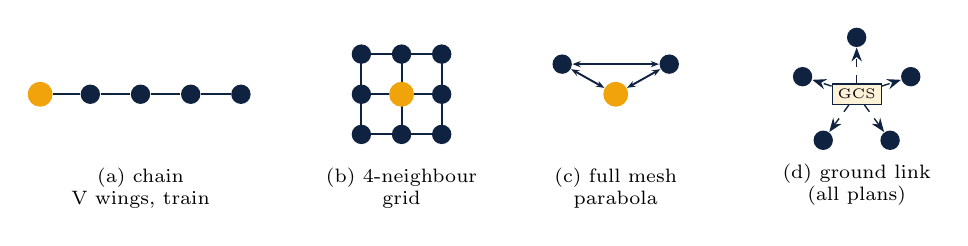
\begin{tikzpicture}[scale=0.85]
  % chain
  \begin{scope}
    \node[leader] (c0) at (0,0) {};
    \foreach \i in {1,...,4} \node[drone] (c\i) at (\i*0.75,0) {};
    \draw[link] (c0)--(c1)--(c2)--(c3)--(c4);
    \node[font=\scriptsize,align=center] at (1.5,-1.4) {(a) chain\\V wings, train};
  \end{scope}
  % grid 4-neighbour
  \begin{scope}[xshift=4.8cm,yshift=0.6cm]
    \foreach \r in {0,1,2} \foreach \c in {0,1,2} \coordinate (q\r\c) at (\c*0.6,-\r*0.6);
    \foreach \r in {0,1,2} \draw[link] (q\r0)--(q\r2);
    \foreach \c in {0,1,2} \draw[link] (q0\c)--(q2\c);
    \foreach \r in {0,1,2} \foreach \c in {0,1,2} \node[drone] at (q\r\c) {};
    \node[leader] at (q11) {};
    \node[font=\scriptsize,align=center] at (0.6,-2.0) {(b) 4-neighbour\\grid};
  \end{scope}
  % full mesh
  \begin{scope}[xshift=8.6cm]
    \node[leader] (m0) at (0,0) {};
    \node[drone] (m1) at (-0.8,0.45) {};
    \node[drone] (m2) at (0.8,0.45) {};
    \draw[link,{Stealth[length=3pt]}-{Stealth[length=3pt]}] (m0)--(m1);
    \draw[link,{Stealth[length=3pt]}-{Stealth[length=3pt]}] (m0)--(m2);
    \draw[link,{Stealth[length=3pt]}-{Stealth[length=3pt]}] (m1)--(m2);
    \node[font=\scriptsize,align=center] at (0,-1.4) {(c) full mesh\\parabola};
  \end{scope}
  % ground star
  \begin{scope}[xshift=12.2cm]
    \node[rectangle,draw=navy,fill=softamber,font=\tiny,inner sep=2pt] (g) at (0,0) {GCS};
    \foreach \a in {0,72,144,216,288} { \node[drone] (s\a) at (\a+90:0.85) {}; \draw[darr,line width=0.5pt] (g)--(s\a); }
    \node[font=\scriptsize,align=center] at (0,-1.35) {(d) ground link\\(all plans)};
  \end{scope}
\end{tikzpicture}
\end{adjustbox}
\caption[Communication topologies]{Communication topologies. (a)--(c) are drone-to-drone relations declared in PDDL;
(d) is the ground-controller link represented by \code{communication-ok}.}
\label{fig:topologies}
\end{figure}

\section{The Range-Checked Link Model of the Parabola Plan}\label{sec:paracomm}
In most plans the links are summarised by the per-drone flag. The parabola plan models each
directed link explicitly. A link from $d_1$ to $d_2$ can be established only when both drones
are airborne at cruise altitude, both radios work, and the straight-line distance between them
is within the communication range of 100\,m:

\begin{lstlisting}
(:action establish-comm-link
    :parameters (?d1 - drone ?d2 - drone)
    :precondition (and (parabola-neighbor ?d1 ?d2) (not (link-up ?d1 ?d2))
                       (airborne ?d1) (airborne ?d2)
                       (at-cruise-altitude ?d1) (at-cruise-altitude ?d2)
                       (communication-ok ?d1) (communication-ok ?d2)
                       (neighbor-comm-ok ?d1) (neighbor-comm-ok ?d2)
                       (<= (link-distance ?d1 ?d2) (comm-range)))
    :effect (link-up ?d1 ?d2))
\end{lstlisting}

\noindent A drone becomes \code{swarm-comm-ready} through \code{confirm-swarm-comm} once it has
a link to every one of its neighbours (a universally quantified condition). Only then can it
take its slot. During flight, \code{hold-parabola-shape} requires every declared link to still be
up, and if a drone loses its neighbour links, \code{detect-neighbor-link-loss} removes all links
to and from that drone, so the shape cannot be re-formed until they are restored. A negative test
with the range reduced to 15\,m (below the 20\,m arm-to-arm distance) correctly produced no plan.
In the solved plan, the six \code{establish-comm-link} actions and three
\code{confirm-swarm-comm} actions appear right after the climbs and before any slot is taken
(Section~\ref{sec:sampleplan}).

\section{Run-Time Communication between Ground Station and Drones}
At run time each drone is an independent thread that owns its state. It can only be reached
through a command inbox and only reports through a telemetry callback. Over the network, the
ground station and drones use a simple JSON-over-UDP protocol, one datagram per message, designed
so that it can later be replaced by MAVLink. Every message carries the drone's
MAVLink SYSID, so one ground socket can address the whole swarm
(Figure~\ref{fig:udp}).

\begin{figure}[H]
\centering
\begin{adjustbox}{max width=\linewidth}
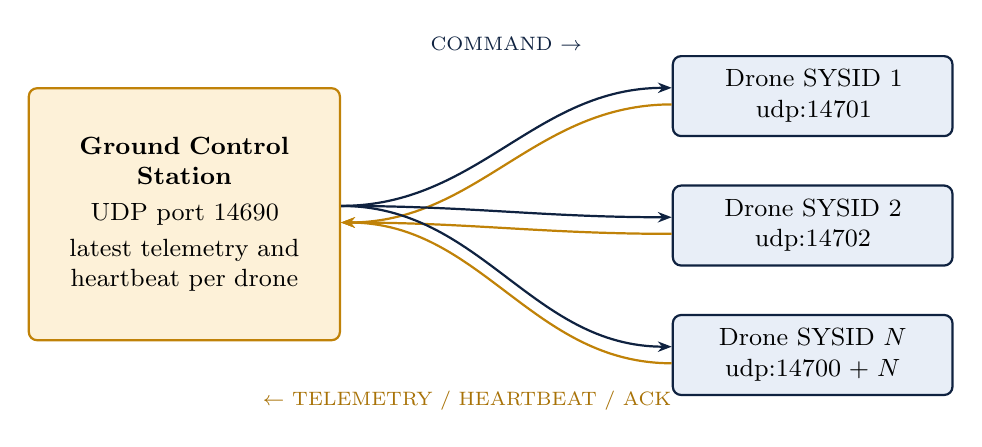
\begin{tikzpicture}[node distance=6mm]
  \node[abox,text width=3.6cm,minimum height=3.2cm] (gcs) {\textbf{Ground Control}\\\textbf{Station}\\[2pt]UDP port 14690\\[2pt]
     latest telemetry and heartbeat per drone};
  \node[box,right=4.2cm of gcs,yshift=1.5cm,text width=3.2cm] (d1) {Drone SYSID 1\\udp:14701};
  \node[box,below=6mm of d1,text width=3.2cm] (d2) {Drone SYSID 2\\udp:14702};
  \node[box,below=6mm of d2,text width=3.2cm] (dn) {Drone SYSID $N$\\udp:$14700+N$};
  \foreach \d in {d1,d2,dn} {
    \draw[arr] ([yshift=3pt]gcs.east) to[out=0,in=180] node[pos=0.55,above,font=\tiny,sloped]{} ([yshift=3pt]\d.west);
    \draw[arr,amber!80!black] ([yshift=-3pt]\d.west) to[out=180,in=0] ([yshift=-3pt]gcs.east);
  }
  \node[font=\scriptsize,navy,align=center] at ($(gcs.north east)!0.5!(d1.north west)+(0,0.35)$) {COMMAND $\rightarrow$};
  \node[font=\scriptsize,amber!70!black,align=center] at ($(gcs.south east)+(1.6,-0.75)$) {$\leftarrow$ TELEMETRY / HEARTBEAT / ACK};
\end{tikzpicture}
\end{adjustbox}
\caption[Ground-station messaging]{Run-time messaging. Commands are routed to a port derived from each drone's SYSID;
every drone reports back to one ground station socket.}
\label{fig:udp}
\end{figure}

\noindent Table~\ref{tab:commands} lists the commands. A drone sends a heartbeat every second
and telemetry every 0.5\,s. The ground station treats a drone as out of contact if no heartbeat
arrives for 3\,s. On the drone side, if nothing is heard from the ground for more than 5\,s the
drone marks its link \code{DEGRADED}, and after 10\,s \code{LOST}. Link loss is therefore
\emph{observed} from missing messages rather than assumed.

\begin{table}[H]
\caption[Run-time commands]{Commands of the ground-station-to-drone protocol}\label{tab:commands}
\small
\begin{tabularx}{\textwidth}{@{}P{0.40\textwidth}Y@{}}
\toprule
\textbf{\normalfont\small Command} & \textbf{Purpose} \\
\midrule
\cmd{NAVIGATE} & The one mission operation: upload a whole route (approach, loop, laps, depart). \\
\cmd{ARM}, \cmd{DISARM}, \cmd{TAKEOFF}, \cmd{LAND} & Enable motors, disable motors, take off or land. \\
\cmd{HOLD}, \cmd{RESUME} & Pause and continue the mission (used while the operator decides on a fault). \\
\cmd{RETURN\_TO\_LAUNCH}, \cmd{ABORT} & Return to the launch point, or stop the mission. \\
\cmd{SET\_GPS} & Fault injection: switch the drone's GPS fix off or on. \\
\cmd{SET\_SPEED} & Change cruise speed in flight. \\
\cmd{TRAIN\_PACE} & Formation keeping: the shared, time-stamped pace of the train or show clock. \\
\cmd{PING}, \cmd{SHUTDOWN} & Liveness check and stop the drone thread. \\
\bottomrule
\end{tabularx}
\end{table}

\section{On-Board Formation Keeping}
A formation needs a shared idea of progress. If the ground station repeatedly
sends late speed corrections, a follower may speed up too much, brake too late
and crowd the drone ahead. This work uses a shared pace and a small correction
loop inside each simulated drone (Figure~\ref{fig:pace}).
\begin{enumerate}
\item \textbf{Receive the pace.} The ground station sends the reference progress,
reference speed and time stamp in a \cmd{TRAIN\_PACE} message.
\item \textbf{Find the assigned position.} Each drone updates the reference for
the elapsed time and subtracts its own distance behind the leader. For example,
a follower assigned one spacing behind aims for one spacing less path progress.
\item \textbf{Compare with actual progress.} The drone measures how far it has
travelled along its own route. If it is behind its target, it may increase speed;
if it is ahead, it slows down.
\item \textbf{Respect the drone ahead.} A reported small front gap limits any
speed increase. The ground station can slow the common pace for a lagging drone.
This depends on reported information and does not guarantee collision avoidance.
\end{enumerate}
For star and planetary shows, the reference is a shared show clock. Each drone
has a timetable telling it where to be at each phase. Using the same clock helps
all drones start and finish a shape change together. This local speed controller
follows a prepared route; it does not create a new PDDL mission after a fault.

\begin{figure}[H]
\centering
\begin{adjustbox}{max width=\linewidth}
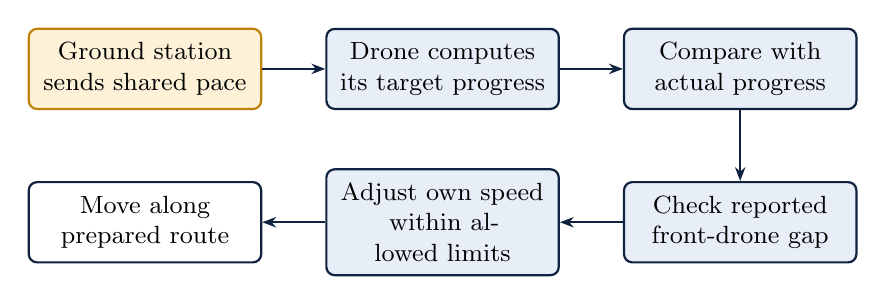
\begin{tikzpicture}[node distance=9mm and 8mm]
\node[abox,text width=2.6cm] (g) {Ground station\\sends shared pace};
\node[box,right=of g,text width=2.6cm] (t) {Drone computes\\its target progress};
\node[box,right=of t,text width=2.6cm] (e) {Compare with\\actual progress};
\node[box,below=of e,text width=2.6cm] (c) {Check reported\\front-drone gap};
\node[box,left=of c,text width=2.6cm] (v) {Adjust own speed\\within allowed limits};
\node[gbox,left=of v,text width=2.6cm] (m) {Move along\\prepared route};
\draw[arr] (g)--(t);\draw[arr] (t)--(e);\draw[arr] (e)--(c);
\draw[arr] (c)--(v);\draw[arr] (v)--(m);
\end{tikzpicture}
\end{adjustbox}
\caption[Local formation control]{On-board formation keeping. Only the pace is sent from the ground; each drone closes its
own gap every tick.}
\label{fig:pace}
\end{figure}

\section{How the Two Levels Relate}
The PDDL flags are a \emph{planning-time} statement: the plan is only valid under the assumption
that the listed links work. The run-time protocol is what actually carries commands and reports.
The two are connected through the fault events of Chapter~\ref{ch:faults}: when the run time
observes a fault, the mission is held and the operator decides how to continue. The PDDL
conditions do not by themselves monitor real radio links; this distinction is discussed in
Chapter~\ref{ch:discussion}.

%% =====================================================================
%%  CHAPTER 7  FAULTS AND BATTERY HEALTH
%% =====================================================================
\chapter{Fault Modelling and Battery Health}\label{ch:faults}

\section{Simple Fault Examples}
A fault means that a condition needed for the mission is no longer true.
These examples illustrate existing rules; they do not add unimplemented recovery behaviour.
\begin{itemize}
\item \textbf{GPS is lost.} A drone no longer has a reliable position fix. The
GPS condition fails, so the model cannot continue its normal move. In the
simulator, the operator can hold the mission and decide what to do next.
\item \textbf{A controller message is missing.} Missing heartbeats can indicate
lost contact. The ground station reports the problem; a neighbour fact in PDDL
cannot restore the connection.
\item \textbf{A formation neighbour is unavailable.} The formation no longer
meets its assumed readiness conditions. The plan has no automatic action that
redesigns the formation around the missing member.
\item \textbf{Battery is low.} A proposed leg may need more energy than is
available. Planning checks can reject the leg; during flight the low-battery
warning asks the operator to decide whether to land.
\end{itemize}
The common sequence is: recognise the problem, stop relying on the failed
condition, notify the controller, and choose an available response. Changing a
PDDL state flag does not itself make a physical drone stop or repair the fault.

\section{Faults Modelled in PDDL}
Every domain includes the same family of detection actions. Each one fires for a flying drone
whose health flag has failed, records a failure state, and takes the drone out of flight and,
in formation plans, out of the formation. Table~\ref{tab:faults} lists them.

\begin{table}[H]
\caption[Fault detection actions]{Fault detection actions shared by the domains}\label{tab:faults}
\small
\begin{tabularx}{\textwidth}{@{}P{0.40\textwidth}P{0.22\textwidth}Y@{}}
\toprule
\textbf{\normalfont\small Action} & \textbf{Fires when} & \textbf{Effect} \\
\midrule
detect-gps-loss & flying and not \code{gps-ok} & \code{gps-lost}; not flying; leaves the
formation (travel also sets \code{gps-warning}) \\
detect-communication-loss & flying and not \code{communication-ok} & \code{communication-lost};
not flying; leaves the formation; parabola also clears \code{swarm-comm-ready} \\
detect-neighbor-link-loss & flying and not \code{neighbor-comm-ok} (formation plans) &
\code{communication-lost}; leaves the formation; parabola also drops every link to and from the
drone \\
detect-health-failure & flying and \code{health} $<$ \code{minimum-health} (40) &
\code{health-failure}; not flying; leaves the formation \\
notify-ground-controller & any of the three failure states & \code{controller-notified} \\
\bottomrule
\end{tabularx}
\end{table}

The GPS loss detection, for example, is:

\begin{lstlisting}
(:action detect-gps-loss
    :parameters (?d - drone)
    :precondition (and (flying ?d) (not (gps-ok ?d)))
    :effect (and (gps-lost ?d) (not (flying ?d)) (not (in-formation ?d))))
\end{lstlisting}

\noindent Because every movement and formation action also requires \code{gps-ok},
\code{communication-ok}, \code{drone-healthy} and, for formations, \code{neighbor-comm-ok}, a
problem that starts with a failed flag has no plan that moves the affected drone. The planner
thus refuses to fly an unhealthy drone, and a failed member blocks the formation actions that
depend on it.

\section{Ground Controller Responses}
The point-to-point domain goes further and models what the ground controller can order once it
has been notified (Figure~\ref{fig:faultflow}):
\begin{itemize}
  \item \textbf{Return}: \code{controller-order-return} sets \code{emergency-return}, and
        \code{return-to-source} flies the drone back over a safe route, provided the battery
        covers the return leg.
  \item \textbf{Hover}: \code{controller-order-hover} puts the drone in a hover. The \code{hover}
        action drains \code{hover-energy} while the battery stays above the return reserve; when
        it reaches the reserve, \code{initiate-low-battery-return} switches the drone to an
        emergency return.
  \item \textbf{Sacrifice}: \code{sacrifice-drone} lands the drone immediately where it is when the
        controller decides it cannot be recovered.
\end{itemize}

\begin{figure}[H]
\centering
\begin{adjustbox}{max width=\linewidth}
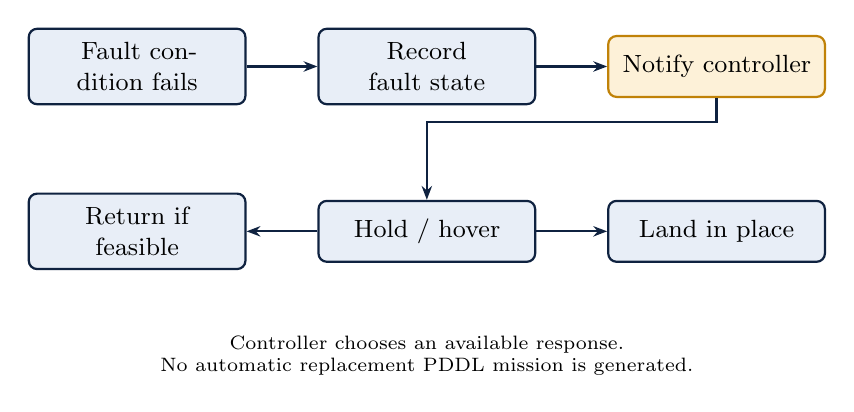
\begin{tikzpicture}[node distance=8mm and 9mm]
\node[box,text width=2.4cm] (f) {Fault condition fails};
\node[box,right=of f,text width=2.4cm] (d) {Record fault state};
\node[abox,right=of d,text width=2.4cm] (n) {Notify controller};
\node[box,below=12mm of d,text width=2.4cm] (h) {Hold / hover};
\node[box,left=of h,text width=2.4cm] (r) {Return if feasible};
\node[box,right=of h,text width=2.4cm] (l) {Land in place};
\draw[arr] (f)--(d);\draw[arr] (d)--(n);
\draw[arr] (n.south)--++(0,-0.3)-|(h.north);
\draw[arr] (h)--(r);\draw[arr] (h)--(l);
\node[font=\scriptsize,align=center,below=8mm of h] {Controller chooses an available response.\\No automatic replacement PDDL mission is generated.};
\end{tikzpicture}
\end{adjustbox}
\caption[Fault response sequence]{Fault handling in the point-to-point domain: detection, notification and the three
controller responses.}
\label{fig:faultflow}
\end{figure}

\section{Battery as a Planning Resource}
Battery is a numeric fluent in every domain, in model units with 100 as a full charge. It is used
in three ways.

\paragraph{Energy per leg}
Each leg has an \code{energy-required} value. When a template is retargeted, this value is
recomputed from the new leg length at the leg's own energy-per-metre rate, with a default of
0.0125 units per metre (12.5 units per kilometre). Every move requires the battery to be
strictly greater than the leg's cost and decreases it by that cost.

\paragraph{Climb, cruise and hover energy}
Formation plans charge \code{climb-energy} for the climb to cruise altitude (in the parabola
plan 4 units for the vertex and 5 for the arms, which climb 10\,m further), and
\code{cruise-leg-energy} (12 units) for each follower or arm leg. The travel domain charges
\code{hover-energy} for each hover step.

\paragraph{Reserve for return}
Each template uses a return reserve of 30 planning units. Pre-flight checks
require enough charge before launch. The relevant leg checks decide whether
the next move can be afforded; hover and search models include return behaviour
when the reserve is reached. Health is a separate
numeric score (100 initially, minimum 40), so a drone can be refused for poor health even with a
full battery.

\section{Battery Health at Run Time}
During flight each drone thread integrates its own battery. With the default settings a drone has
a 5\,200\,mAh battery and draws a nominal 20\,A in flight; its percentage is computed from the
consumed charge. The drone classifies its own health from the battery and the GPS fix
(Figure~\ref{fig:battery}): \code{NOMINAL} above 20\,\%, \code{DEGRADED} at or below 20\,\% or
without GPS, \code{CRITICAL} at or below 5\,\%, and \code{FAILED} if the battery is exhausted in
flight, in which case the drone is lost.

\begin{figure}[H]
\centering
\begin{adjustbox}{max width=\linewidth}
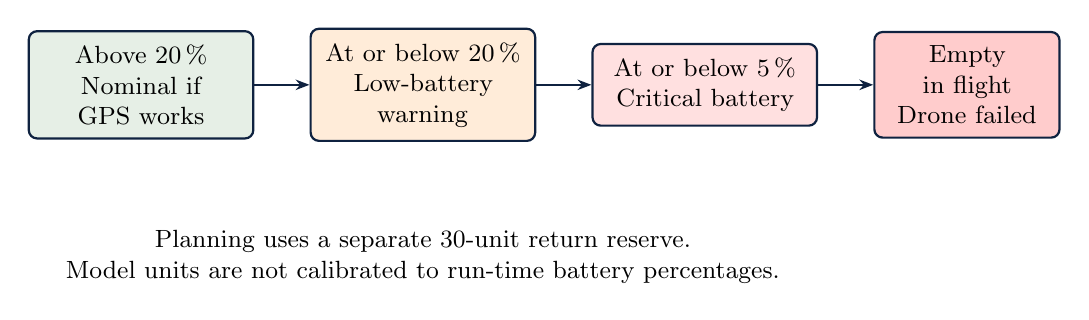
\begin{tikzpicture}[node distance=7mm]
\node[box,fill=okgreen!12,text width=2.5cm] (n) {Above 20\,\%\\Nominal if GPS works};
\node[box,fill=orange!15,right=of n,text width=2.5cm] (l) {At or below 20\,\%\\Low-battery warning};
\node[box,fill=red!12,right=of l,text width=2.5cm] (c) {At or below 5\,\%\\Critical battery};
\node[box,fill=red!20,right=of c,text width=2cm] (f) {Empty in flight\\Drone failed};
\draw[arr] (n)--(l);\draw[arr] (l)--(c);\draw[arr] (c)--(f);
\node[font=\small,align=center,below=10mm of l] {Planning uses a separate 30-unit return reserve.\\Model units are not calibrated to run-time battery percentages.};
\end{tikzpicture}
\end{adjustbox}
\caption[Battery states and reserve]{Run-time battery states. A low-battery event
pauses the mission for an operator decision. The PDDL reserve is a separate
planning quantity, rather than a calibrated percentage threshold.}
\label{fig:battery}
\end{figure}

\noindent When any drone crosses the low-battery threshold, the ground station \emph{pauses the
whole mission} so that the drones do not drain while the operator decides; at the compressed time
scale the decision window would otherwise be a fraction of a second. A dialog shows the drone's
battery and the nearest landing point, with a note whether it is within reach on the remaining
charge. The operator may divert and land now, or press on, in which case the drone will be lost
when the battery runs flat. A drone whose battery reaches zero in flight is reported as lost and
sacrificed.

\section{Fault Injection and Operator Decisions}
The GUI's fault injection panel lets the operator target one or more drones by SYSID with a
fault type (GPS loss, communications loss or battery failure), a severity and a duration
(zero meaning until reset). In the thread-based backend, GPS loss is delivered as a
\code{SET\_GPS} command, so the drone itself loses its fix. On GPS loss the ground station holds
the swarm and asks the operator whether the drone should fall back to its start point and land,
showing the distance back and whether the remaining charge covers it; otherwise the drone holds
position until GPS returns, while its battery keeps draining. When GPS is reacquired the mission
resumes. Table~\ref{tab:faultmap} maps each fault to its PDDL model and run-time behaviour.

\begin{table}[H]
\caption[Faults and run-time responses]{Faults: how each is modelled in PDDL and handled at run time}\label{tab:faultmap}
\small
\begin{tabularx}{\textwidth}{@{}P{0.17\textwidth}P{0.32\textwidth}Y@{}}
\toprule
\textbf{Fault} & \textbf{PDDL model} & \textbf{Run-time behaviour} \\
\midrule
GPS loss & not \code{gps-ok}; \code{detect-gps-loss} & injected with \code{SET\_GPS}; drone
\code{DEGRADED}; swarm held; operator chooses fall-back or hold \\
Communication loss & not \code{communication-ok}; \code{detect-communication-loss} & observed
from missing heartbeats and contact (\code{DEGRADED} after 5\,s, \code{LOST} after 10\,s) \\
Neighbour link loss & not \code{neighbor-comm-ok}; \code{detect-neighbor-link-loss} & reflected
in formation keeping through the front-drone cap and pace slowing \\
Health failure & \code{health} below \code{minimum-health}; \code{detect-health-failure} &
drone health classes \code{NOMINAL}/\code{DEGRADED}/\code{CRITICAL}/\code{FAILED} \\
Low battery & battery not above reserve; {\small\code{notify-insufficient-battery}},
\code{initiate-low-battery-return} & at 20\,\% swarm paused, operator chooses emergency landing
or press on; at 0\,\% drone lost \\
\bottomrule
\end{tabularx}
\end{table}

%% =====================================================================
%%  CHAPTER 8  RESULTS
%% =====================================================================
\chapter{Verification and Results}\label{ch:results}

\section{Method}
Each plan was verified in two ways. First, ENHSP was run directly on problems produced by the real
expand, retarget and solve pipeline, for a range of drone counts. Second, the resulting routes were
flown without the GUI through the drone threads, and the spacing, altitudes
and landing positions were measured. Negative tests were added where a plan must refuse a
problem. The run logs in \code{plans/*/runs/} record the in-app requests.

\section{In-App Planning Requests}
Table~\ref{tab:runs} summarises the logged requests for the four longest-running plans. Every
unsolvable travel and V request was traced to an infeasible combination of source, destination
and no-fly area, where no safe path existed. The grid failures all occurred in a short window
before a template fix (Section~\ref{sec:defects}); every grid request after the fix solved.

\begin{table}[H]
\caption[Planning request records]{Logged planning requests per plan}\label{tab:runs}
\small
\begin{tabularx}{\textwidth}{@{}lrrrY@{}}
\toprule
\textbf{Plan} & \textbf{Runs} & \textbf{Solved} & \textbf{Unsolvable} & \textbf{Notes} \\
\midrule
Forest search & 69 & 69 & 0 & no failures on record \\
Travel        & 83 & 76 & 7 & infeasible no-fly inputs during early testing \\
V formation   & 65 & 62 & 2 & 2 infeasible inputs; 1 run closed mid-plan \\
Grid          & 19 & 15 & 4 & all 4 before the hover-altitude fix \\
\bottomrule
\end{tabularx}
\end{table}

\section{Scalability of the Cube Formation}
Table~\ref{tab:cube} and Figure~\ref{fig:cubeplot} show planning time and plan length for the
cube formation. Plan length grows linearly with the number of drones, about four actions per
drone. Planning time stays below 4\,s up to 36 drones and reaches 50\,s for a full $4\times4\times4$
block of 64 drones. A launch-order audit of the 25-drone plan found no drone taking off before
its layer opened and no layer opening before the one below had finished climbing.

\begin{table}[H]
\caption[Cube planning results]{Cube formation: ENHSP results through the real pipeline}\label{tab:cube}
\small
\begin{tabular*}{\textwidth}{@{\extracolsep{\fill}}lrrrrrrrr@{}}
\toprule
\textbf{Drones} & 8 & 9 & 12 & 16 & 25 & 27 & 36 & 64 \\
\textbf{Shape} & $2{\times}2{\times}2$ & $3{\times}2{\times}2$ & $2{\times}3{\times}3$ & $2{\times}3{\times}3$ &
 $3{\times}3{\times}3$ & $3{\times}3{\times}3$ & $3{\times}4{\times}4$ & $4{\times}4{\times}4$ \\
\midrule
Time (s) & 0.4 & 0.5 & 0.6 & 0.7 & 1.2 & 1.8 & 3.4 & 50.0 \\
Plan length & 42 & 47 & 58 & 74 & 111 & 119 & 155 & 268 \\
\bottomrule
\end{tabular*}
\end{table}

\begin{figure}[H]
\centering
\begin{adjustbox}{max width=\linewidth}
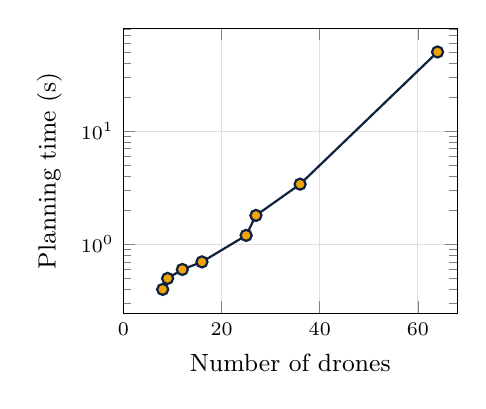
\begin{tikzpicture}
\begin{axis}[
  width=0.48\textwidth,height=5.2cm,
  xlabel={Number of drones},ylabel={Planning time (s)},
  ymode=log,log basis y=10,
  grid=major,grid style={gray!25},
  tick label style={font=\scriptsize},label style={font=\small},
  xmin=0,xmax=68,
]
\addplot[navy,thick,mark=*,mark options={fill=amber,draw=navy}] coordinates
  {(8,0.4)(9,0.5)(12,0.6)(16,0.7)(25,1.2)(27,1.8)(36,3.4)(64,50.0)};
\end{axis}
\end{tikzpicture}
\end{adjustbox}\hfill
\begin{adjustbox}{max width=\linewidth}
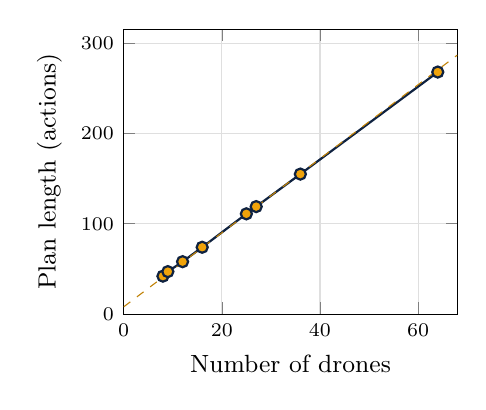
\begin{tikzpicture}
\begin{axis}[
  width=0.48\textwidth,height=5.2cm,
  xlabel={Number of drones},ylabel={Plan length (actions)},
  grid=major,grid style={gray!25},
  tick label style={font=\scriptsize},label style={font=\small},
  xmin=0,xmax=68,ymin=0,
]
\addplot[navy,thick,mark=*,mark options={fill=amber,draw=navy}] coordinates
  {(8,42)(9,47)(12,58)(16,74)(25,111)(27,119)(36,155)(64,268)};
\addplot[amber!80!black,dashed,domain=0:68] {4.1*x+8};
\end{axis}
\end{tikzpicture}
\end{adjustbox}
\caption[Cube planning scalability]{Cube formation scalability. Left: planning time (log scale). Right: plan length, close to
linear in the number of drones (dashed line $\approx 4.1N + 8$).}
\label{fig:cubeplot}
\end{figure}

\section{Figure-Eight Capacity and Flight Quality}
On an asymmetric eight with lobes of 337\,m and 281\,m, the computed capacity was 27 drones. ENHSP
solved every count up to 27 and returned no plan for 28, in agreement with the Python check
(Table~\ref{tab:fig8}). With a full 27-drone train, the minimum distance between any two drones at
any waypoint step was 9.85\,m, including at the crossing. Ten drones with 20 laps solved in 0.8\,s,
because laps are counted in PDDL and flown on board with a single repeat instruction rather than
being unrolled.

\begin{table}[H]
\caption[Figure-eight capacity]{Figure-eight train: ENHSP results on an eight of capacity 27}\label{tab:fig8}
\small
\begin{tabular*}{\textwidth}{@{\extracolsep{\fill}}lrrrrrr@{}}
\toprule
\textbf{Drones} & 2 & 5 & 12 & 25 & 27 & 28 \\
\midrule
Time (s) & 0.4 & 0.4 & 0.7 & 2.7 & 3.3 & -- \\
Plan length & 26 & 38 & 66 & 118 & 126 & no plan (as intended) \\
\bottomrule
\end{tabular*}
\end{table}

\noindent After formation keeping moved on board (Chapter~\ref{ch:comm}), a replay of a logged
16-drone, 2-lap run changed from a median neighbour gap of 23.7\,m with a minimum of 0.0\,m
(collisions) to a median of 10.0\,m, with 90\,\% of samples between 9.2 and 10.8\,m, and every
drone landed on its own pad.

\section{Other Plans}
Table~\ref{tab:other} summarises the verification of the remaining plans.

\begin{table}[H]
\caption[Other mission checks]{Verification summary of the remaining plans}\label{tab:other}
\small
\begin{tabularx}{\textwidth}{@{}lY@{}}
\toprule
\textbf{Plan} & \textbf{Result} \\
\midrule
V formation & 3-, 5- and 7-drone V's solve through the real pipeline after the neighbour chain was
added. \\
Parabola & 27-step plan with a detour, about 0.03--0.1\,s. Negative checks (arm at 55\,m, flat
50\,m line, communication range 15\,m) give no plan. In flight, altitudes held at 50/60/60\,m,
vertex--arm gap 14.1--15.0\,m on a straight 1\,km route. \\
Star show & 6 drones $\times$ 1 lap 0.3\,s; 40 drones $\times$ 5 laps 0.6\,s. In flight (10
drones, 2 laps), worst drone 0.7--3.2\,m off its slot while shapes were held, closest pair
9.3\,m, every drone landed on its own pad. \\
Planets & 2--8 drones $\times$ 3 laps, 0.2--0.3\,s. With 8 drones every drone stayed within 0.4\,m
of its orbit and turned the correct direction and number of turns. \\
Road inspection & 1.4\,km and 3.8\,km real roads followed with no measurable deviation from the
road line; ENHSP 0.3\,s; a source 393\,m off the road was correctly refused. \\
\bottomrule
\end{tabularx}
\end{table}

\section{Reading a Parabola Plan}\label{sec:sampleplan}
The parabola result follows a clear dependency order. Each drone first passes
its checks, takes off and reaches its own cruise height. The planner then
establishes the directed links and confirms that every drone can reach its
required neighbours. Slot assignment is allowed only after that confirmation.
The formation is established, cruises each planned leg, restores its shape at
the next location, and finally records mission completion. The selected
communication facts in Chapter~\ref{ch:plans} and the link action in
Section~\ref{sec:paracomm} explain the important parts without repeating the full output.

\section{Defects Found and Fixed}\label{sec:defects}
Verification found several modelling defects. They are recorded here because each one taught a
general lesson about writing PDDL for a template-expanding pipeline.

\begin{table}[H]
\caption[Modelling fixes]{Modelling defects found during verification}\label{tab:defects}
\small
\begin{tabularx}{\textwidth}{@{}P{0.2\textwidth}P{0.36\textwidth}Y@{}}
\toprule
\textbf{Plan} & \textbf{Defect} & \textbf{Fix and lesson} \\
\midrule
Grid & \code{hover-altitude} facts were written over three lines. The line-by-line cloner copied
only the middle line, leaving the value undefined for every added drone; AIBR then reported any
grid larger than $1\times2$ as unsolvable. & Rewritten as one line per fact. Templates must keep
one fact per line. \\
Cube & Layer gate written as a comparison of two fluents. A 25-drone, 3-layer cube did not solve
in 90\,s. & Replaced by propositional layer objects; solved in 1.2\,s. Prefer propositional
gates for ordering. \\
Cube & A quantified variable \code{?l} in \code{establish-cube-formation} shadowed the action's
location parameter, making every problem unsolvable. & Variable renamed. Never reuse a parameter
name inside a quantifier. \\
V formation & Readiness checked only the ground link; there was no notion of which drones sit
next to each other. & Added \code{wing-neighbor} chain and \code{neighbor-comm-ok}, with
\code{detect-neighbor-link-loss}. \\
Figure-8 & Ground-station correction caused oscillation and collisions in a 16-drone train. &
Formation keeping moved on board with a shared pace (Chapter~\ref{ch:comm}). \\
\bottomrule
\end{tabularx}
\end{table}

%% =====================================================================
%%  CHAPTER 9  DISCUSSION
%% =====================================================================
\chapter{Discussion and Limitations}\label{ch:discussion}

\section{What the Models Check}
An ENHSP plan shows that the written goal can be reached using the allowed
actions and the supplied initial facts. The models can check route permission,
energy conditions, formation readiness and mission-specific ordering rules.
This makes the planning logic visible and reviewable.

The result depends on what is represented. A healthy-link flag is an assumption,
not a radio measurement, and a fixed slot is not a physical collision-avoidance
controller. The simulator must still execute the route and monitor the drones.
A valid symbolic plan therefore does not guarantee that an actual flight will
remain safe after unexpected changes.

\section{Limitations}
The current system is useful for studying mission logic, but the following limits
must be considered before applying its plans outside the simulator.
\begin{itemize}
  \item \textbf{Fixed cruise height.} A drone generally follows its assigned constant
        height during cruise, after take-off and climb. Cube layers and parabola arms
        use different assigned heights. The planner does not choose a changing height
        profile to follow terrain or avoid new obstacles.
  \item \textbf{No automatic replacement plan.} When a plan fails during execution,
        the system does not automatically solve a new PDDL problem for the remaining
        mission. The operator must respond, for example by holding, returning or landing.
  \item \textbf{Mission-specific swarm limits.} Swarm size is configurable for expandable
        missions, but the current parabola and road-inspection missions remain fixed.
        The show limits and figure-eight path capacity must also be respected.
  \item \textbf{Symbolic communication.} The PDDL flags describe the assumed state of the links at
        planning time. They are not updated from live radio measurements during flight; run-time
        faults are handled by the ground station and the operator, not by replanning.
  \item \textbf{Faults are detected, not planned around.} The detection actions record a failure,
        but the goals still require healthy drones, so the planner does not produce contingency
        branches. Online replanning after a fault is left for future work.
  \item \textbf{Battery units.} Battery and energy in PDDL are model units with 100 as full. They
        are not calibrated against the 5\,200\,mAh run-time model, so the planning reserve (30
        units) and the run-time low threshold (20\,\%) are separate safeguards.
  \item \textbf{Fault injection coverage.} The GUI offers GPS loss, communications loss and battery
        failure, but in the thread-based backend only GPS loss is currently delivered to the
        drones; communication loss is observed from missing messages and low battery arises from
        consumption.
  \item \textbf{Grounding cost.} Large two-dimensional grids are expensive to ground: a 16-drone
        ($4\times4$) grid exceeded a 6\,GB heap in local testing, even though larger cubes solve,
        because of the different structure of their quantified conditions.
  \item \textbf{Simulation only.} All results come from the simulator. No physical flight was
        performed, and the road inspection plan depends on an external routing service.
\end{itemize}

%% =====================================================================
%%  CHAPTER 10  CONCLUSION
%% =====================================================================
\chapter{Conclusion and Future Work}\label{ch:conclusion}

\section{Conclusion}
This thesis presented the PDDL planning layer of a drone swarm simulator. Ten mission plans were
built on one shared vocabulary, covering travel, area search, four rigid formations, a
figure-eight train, two shape-changing shows and road inspection. Communication was modelled as
neighbour relations with per-drone flags, and, in the parabola plan, as an explicit mesh of
range-checked links. Faults were modelled as detection actions with ground-controller responses,
and battery as a numeric resource with a return reserve, complemented at run time by thresholds
that pause the swarm and ask the operator.

The plans run through the simulator pipeline: they are retargeted to map inputs,
solved by ENHSP and flown by the drone threads. Expandable missions use the selected
number of drones; the current fixed-size missions retain their stated limits. The results show that
careful modelling keeps planning fast for realistic swarm sizes: 64 drones in a cube in 50\,s,
a 27-drone figure-eight train in 3.3\,s, and most missions in well under a second. The defects
found during verification led to general modelling rules that will help anyone extending the
plans.

\section{Future Work}
\begin{enumerate}
  \item \textbf{Online replanning.} Feed run-time faults back into the PDDL state and replan the
        remaining mission, for example closing a formation around a lost drone.
  \item \textbf{Calibrated energy model.} Derive \code{energy-required} and the reserve from the
        drone's battery capacity, current draw, speed and wind, so that planning and run-time
        thresholds use the same units.
  \item \textbf{A local planner for each drone.} Give every drone its own planner
        to adjust its remaining route using its local state and nearby drones,
        while staying consistent with the swarm mission. The present local speed
        controller follows an existing route; this proposed planner would be able
        to choose a revised route when conditions change.
  \item \textbf{Complete fault injection.} Deliver communication loss and battery failure faults
        to the drone threads, matching the GUI options, and test the operator responses under
        each.
  \item \textbf{Larger grids.} Reduce grounding cost for large two-dimensional grids, for example
        by the same propositional restructuring that made the cube scale.
  \item \textbf{Physical validation.} Validate the planning assumptions with controlled
        physical-drone experiments after simulation checks.
\end{enumerate}

%% =====================================================================
%%  REFERENCES
%% =====================================================================
\clearpage
\phantomsection
\addcontentsline{toc}{chapter}{References}
\renewcommand{\bibname}{References}
\makeatletter\renewcommand\@biblabel[1]{}\makeatother
\begin{thebibliography}{99}
\setlength{\itemsep}{3pt}
\bibitem{mcdermott1998pddl} D. McDermott, M. Ghallab, A. Howe, C. Knoblock, A. Ram, M. Veloso,
  D. Weld and D. Wilkins, \emph{PDDL -- The Planning Domain Definition Language}, Technical Report
  CVC TR-98-003, Yale Center for Computational Vision and Control, 1998.
\bibitem{fox2003pddl21} M. Fox and D. Long, \emph{PDDL2.1: An Extension to PDDL for Expressing
  Temporal Planning Domains}, Journal of Artificial Intelligence Research, vol.~20, pp.~61--124,
  2003.
\bibitem{ghallab2004automated} M. Ghallab, D. Nau and P. Traverso, \emph{Automated Planning:
  Theory and Practice}, Morgan Kaufmann, 2004.
\bibitem{scala2016interval} E. Scala, P. Haslum, S. Thi\'ebaux and M. Ramirez,
  \emph{Interval-Based Relaxation for General Numeric Planning}, Proceedings of the 22nd European
  Conference on Artificial Intelligence (ECAI), pp.~655--663, 2016.
\bibitem{scala2020subgoaling} E. Scala, P. Haslum, S. Thi\'ebaux and M. Ramirez,
  \emph{Subgoaling Techniques for Satisficing and Optimal Numeric Planning}, Journal of Artificial
  Intelligence Research, vol.~68, pp.~691--752, 2020.
\bibitem{chung2018survey} S.-J. Chung, A. A. Paranjape, P. Dames, S. Shen and V. Kumar,
  \emph{A Survey on Aerial Swarm Robotics}, IEEE Transactions on Robotics, vol.~34, no.~4,
  pp.~837--855, 2018.
\bibitem{brambilla2013swarm} M. Brambilla, E. Ferrante, M. Birattari and M. Dorigo,
  \emph{Swarm Robotics: A Review from the Swarm Engineering Perspective}, Swarm Intelligence,
  vol.~7, no.~1, pp.~1--41, 2013.
\bibitem{reynolds1987flocks} C. W. Reynolds, \emph{Flocks, Herds and Schools: A Distributed
  Behavioral Model}, Proceedings of SIGGRAPH '87, Computer Graphics, vol.~21, no.~4, pp.~25--34,
  1987.
\bibitem{dubins1957curves} L. E. Dubins, \emph{On Curves of Minimal Length with a Constraint on
  Average Curvature, and with Prescribed Initial and Terminal Positions and Tangents}, American
  Journal of Mathematics, vol.~79, no.~3, pp.~497--516, 1957.
\bibitem{luxen2011osrm} D. Luxen and C. Vetter, \emph{Real-Time Routing with OpenStreetMap Data},
  Proceedings of the 19th ACM SIGSPATIAL International Conference on Advances in Geographic
  Information Systems, pp.~513--516, 2011.
\bibitem{mavlink} MAVLink Development Team, \emph{MAVLink Micro Air Vehicle Communication
  Protocol}, \url{https://mavlink.io/en/}.
\bibitem{enhsp} E. Scala, \emph{ENHSP -- Expressive Numeric Heuristic Search Planner},
  \url{https://sites.google.com/view/enhsp/}.
\bibitem{pyside6} The Qt Company, \emph{Qt for Python (PySide6)},
  \url{https://doc.qt.io/qtforpython-6/}.
\end{thebibliography}

\end{document}
